\chapter{ทฤษฎีที่เกี่ยวข้อง}

ในบทนี้จะอธิบายถึงองค์ความรู้และทฤษฎีที่จำเป็นต่อการพัฒนาแอปพลิเคชันรวมทั้งงานวิจัยที่เกี่ยวข้อง มีรายละเอียดดังนี้

\begin{enumerate}[label=2.\arabic*]
	\item แนวคิดทฤษฏีที่เกี่ยวข้อง
	\begin{enumerate}[label=2.1.\arabic*]
		\item Hybrid Mobile Application
		\item ความรู้พื้นฐานระบบปฏิบัติการแอนดรอยด์
		\item ความรู้พื้นฐานของระบบปฏิบัติการไอโอเอส
		\item ความรู้พื้นฐาน Ionic Framework
		\item การใช้งาน Firebase เป็นฐานข้อมูล
		\item Dialogflow
		\item Libraries moment.js
		\item Google Maps API
	\end{enumerate}
	\item เอกสารและงานวิจัยที่เกี่ยวข้อง
\end{enumerate}

\section{แนวคิดทฤษฏีที่เกี่ยวข้อง}

% Hybrid Application

\subsection{Hybrid Mobile Application}
Hybrid Application คือ แอปพลิเคชันที่ถูกพัฒนาขึ้นมาเพื่อให้สามารถทำงานได้บนระบบปฏิบัติการทั้งหมดโดยพัฒนาแค่ครั้งเดียว 
โดยจำเป็นต้องผ่านเฟรมเวิร์คต่างๆเพื่อให้สามารถทำงานบน OS นั้นๆได้ เช่น PhoneGap (โฟนเคป) ซึ่งเป็น Open source framework 
ด้วยการพัฒนาแอปด้วยเทคโนโลยีเว็บ html, CSS และ Java Script เป็นต้น 

\begin{figure}[H]
	\centering
	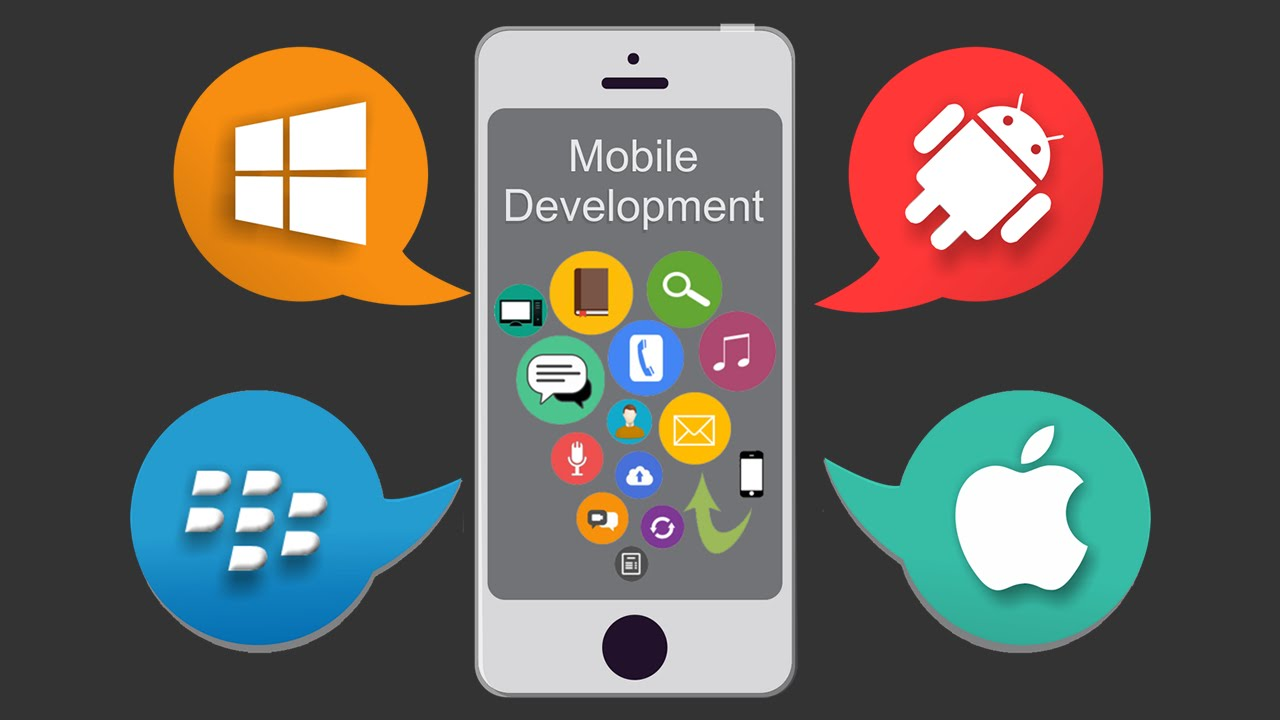
\includegraphics[width=0.5\columnwidth]{Figures/2/hybrid}
	\caption{Hybrid Mobile Application คืออะไร}{ที่มา :  https://www.mindphp.com/คู่มือ/73-คืออะไร/3663-hybrid-application-ไฮบริด-แอปพลิเคชัน-หรือ-hybrid-app-ไฮบริด-แอพ-คืออะไร.html}
	\label{Fig:hybrid}
\end{figure}

การพัฒนา Mobile Application แต่เดิมนั้น ถ้าจะเริ่มก็คงตั้งแต่ยุค J2ME อาจจะเก่ามากจนมาถึงยุคสมัยของ IOS และ Android 
รวมไปถึงน้องสุดท้องอย่าง Windows Phone 
ซึ่งแต่ก่อนก็มีพัฒนาจาก Window CE มาก่อนหน้านี้ จนผู้ใช้ของแต่ละฝั่ง platform เริ่มมีความสำคัญใกล้เคียงกัน ดังนั้น การพัฒนาแอป
เฉพาะของ iOS หรือ Android เพียงอย่างเดียวถือเป็นการเสียโอกาสทางธุรกิจเป็นอย่างมาก จนมีคนเริ่มคิดหาวิธีทำให้ชีวิตง่ายขึ้นโดยการเขียน 
HTML5 + CSS3 + JavaScript แล้วใช้วิธีทำงานผ่าน Web View Component เป็นส่วนของหน้าเบราเซอร์ในแอปอีกที ของแต่ละ Platform 
จนกลายมาเป็นโครงการ Cordova และได้มีการพัฒนาส่วนขยาย Plug-In เพิ่มเรื่อยๆ ทำให้ปัจจุบันเราสามารถเข้าถึง Hardware หรือ Sensor 
ซึ่งโดยปกติ HTML5 ธรรมดาไม่สามารถเข้าถึงได้ 

\begin{figure}[H]
	\centering
	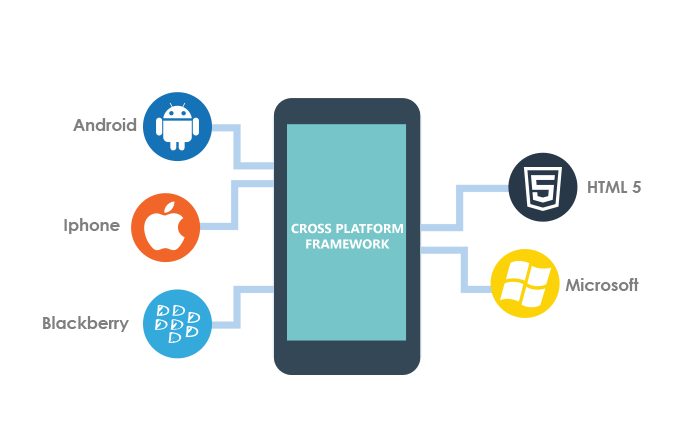
\includegraphics[width=0.5\columnwidth]{Figures/2/hybrid2}
	\caption{Cross Platform Frameworks}{ที่มา :  https://www.promaticsindia.com/mobile-app-development-services/cross-platform-frameworks}
	\label{Fig:hybrid2}
\end{figure}

การเขียนแอปแบบ Hybrid Application คือ การพัฒนาโดยอาศัย Framwork หรือ SDK 
ที่ถูกสร้างมาจากหลากหลายภาษาและมีเครื่องมือที่เหมาะสมกับ Framwork หรือ SDK นั้น ๆ ให้เลือกใช้ในการพัฒนาที่หลากหลายตัวอย่างเช่น 
codova SDK ใช้ ภาษา LUA , Acrobat AIR ใช้ภาษา ACTION SCRIPT 3 หรือ UNITY ใช้ C# และ JAVASCRIPT 
ซึ่งการเขียนในรูปแบบนี้เราสามารถแปลงไปใช้กับระบบปฏิบัติการอื่น ๆ ได้และใช้เวลาน้อยในการเพื่อพัฒนาหลาย ๆ แอปพลิเคชัน

	ข้อดีของ Hybrid Mobile Application
	\begin{enumerate}[label=\arabic*)]
		\item พัฒนาด้วยภาษา HTML, CSS และ JavaScript ทำให้ง่ายและเรียนรู้ได้อย่างรวดเร็ว
		\item พัฒนาครั้งเดียวสามารถใช้ได้หลาย Platform ทั้ง iOS, Android และ Window Phone
		\item ใช้ต้นทุนในการพัฒนาน้อยกว่า Native App
	\end{enumerate}

	ข้อเสียของ Hybrid Mobile Application
	\begin{enumerate}[label=\arabic*)]
		\item ประสิทธิภาพการทำงานจะด้อยกว่า Native App
		\item ในบางกรณีอาจจะใช้ความสามารถของอุปกรณ์ได้ไม่เต็มที่ เนื่องจากต้องขึ้นอยู่กับ Framework ที่เลือกในการพัฒนานั้นมี Component ที่ต้องการหรือไม่
		ดังนั้น Hybrid App จึงมีจุดเด่นในเรื่องความง่ายและพัฒนาได้รวดเร็ว และ Cross-Platforms คือพัฒนาครั้งเดียวแต่สามารถนำไปติดตั้งในหลาย Platforms แต่เมื่อพูดถึงเรื่องประสิทธิภาพในการทำงาน เช่นความเร็ว หรือการเรียกใช้หรือติดต่อ feature ต่าง ๆ ของอุปกรณ์ ก็ต้องยอมรับว่าอาจจะยังด้อยกว่าแอปพลิเคชันที่พัฒนาด้วย Native App ในบางลักษณะการทำงานอยู่ดี
	\end{enumerate}

% Android Studio

\subsection{ความรู้พื้นฐานระบบปฏิบัติการแอนดรอยด์}
แอนดรอยด์ (Android) คือระบบปฏิบัติการแบบเปิดเผยซอร์ฟแวร์ต้นฉบับ (Open Source) โดยบริษัท กูเกิ้ล (Google Inc.) ที่ได้รับความนิยมเป็นอย่างสูง เนื่องจากอุปกรณ์ที่ใช้ระบบปฏิบัติการแอนดรอยด์ มีจำนวนมาก อุปกรณ์มีหลากหลายระดับ หลายราคา รวมทั้งสามารถทำงานบนอุปกรณ์ที่มีขนาดหน้าจอ และความละเอียดแตกต่างกันได้ ทำให้ผู้บริโภคสามารถเลือกได้ตามต้องการและหากมองในทิศทางสำหรับนักพัฒนาโปรแกรม (Programmer) แล้วนั้นการพัฒนาโปรแกรมเพื่อใช้งานบนระบบปฏิบัติการแอนดรอยด์ ไม่ใช่เรื่องยาก เพราะมีข้อมูลในการพัฒนารวมทั้ง Android SDK (Software Development Kit) เตรียมไว้ให้กับนักพัฒนาได้เรียนรู้ และเมื่อนักพัฒนาต้องการจะเผยแพร่หรือจำหน่ายโปรแกรมที่พัฒนาแล้วเสร็จแอนดรอยด์ก็ยังมีตลาดในการเผยแพร่โปรแกรม Google PlayStore แต่หากจะกล่าวถึงโครงสร้างภาษาที่ใช้ในการพัฒนานั้น สำหรับ Android SDK จะยึดโครงสร้างของภาษาจาวา (Java language) ในการเขียนโปรแกรม เพราะโปรแกรมที่พัฒนามาได้จะต้องทำงานอยู่ภายใต้ Dalvik Virtual Machine เช่นเดียวกับโปรแกรมจาวา ที่ต้องทำงานอยู่ภายใต้ Java Virtual Machine (Virtual Machine เปรียบได้กับสภาพแวดล้อมที่โปรแกรมทำงานอยู่)

	\subsubsection{โครงสร้างของระบบปฏิบัติการแอนดรอยด์} 
	การทำความเข้าใจโครงสร้างของระบบปฏิบัติการแอนดรอยด์ \cite{androidbook1} ถือว่าเป็นสิ่งสำคัญเพราะถ้านักพัฒนาโปรแกรม สามารถมองภาพโดยรวมของระบบได้ทั้งหมด จะสามารถเข้าใจถึงกระบวนการทำงานได้ดียิ่งขึ้น และสามารถนำไปช่วยในการออกแบบโปรแกรมที่ต้องการพัฒนาเพื่อให้เกิดประสิทธิภาพในการทำงาน
	
	\begin{figure}[H]
		\centering
		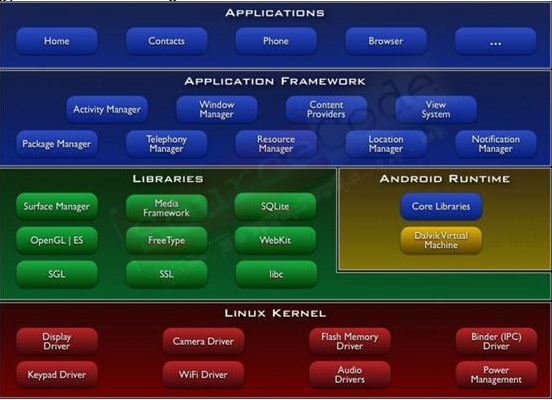
\includegraphics[width=0.8\columnwidth]{Figures/2/androidarchitecture}
		\caption{โครงสร้างของระบบปฏิบัติการแอนดรอยด์}{ที่มา : https://www.theandroid-mania.com/android-architecture/}
		\label{Fig:androidarchitecture}
	\end{figure}
	จากโครงสร้างของระบบปฏิบัติการแอนดรอยด์ในรูปที่ \ref{Fig:androidarchitecture} จะสังเกตได้ว่า มีการแบ่งออกเป็นส่วน ๆ ที่มีความเกี่ยวเนื่องกัน โดยส่วนบนสุดเป็นส่วนที่ผู้ใช้งานทำการติดต่อโดยตรงซึ่งคือส่วนของ Applications ลำดับถัดมาเป็นองค์ประกอบอื่น ๆ ตามลำดับ และสุดท้ายเป็นส่วนที่ติดต่อกับอุปกรณ์โดยผ่านทาง Linux Kernel โครงสร้างของแอนดรอยด์สามารถอธิบายได้ดังนี้

	\begin{enumerate}[label=\arabic*)]
		\item Applications ส่วนแอปพลิเคชันหรือส่วนของโปรแกรมที่มากับระบบปฏิบัติการ หรือเป็นกลุ่มของโปรแกรมที่ผู้ใช้งานได้ทำการติดตั้งไว้ โดยผู้ใช้งานสามารถเรียกใช้โปรแกรมต่าง ๆ ได้โดยตรงซึ่งการทำงานของแต่ละโปรแกรมจะเป็นไปตามที่ผู้พัฒนาโปรแกรมได้ออกแบบและเขียนโค้ด (Code) โปรแกรมเอาไว้
		\item Application Framework  เป็นส่วนที่มีการพัฒนาขึ้นเพื่อให้นักพัฒนาสามารถพัฒนาโปรแกรมได้สะดวก และมีประสิทธิภาพมากยิ่งขึ้น โดยนักพัฒนาไม่จำเป็นต้องพัฒนาในส่วนที่มีความยุ่งยากมากๆ เพียงแค่ทำการศึกษาถึงวิธีการเรียกใช้งาน Application Framework ในส่วนที่ต้องการใช้งานแล้วนำมาใช้งาน ซึ่งมีหลายกลุ่มด้วยกัน ตัวอย่างเช่น
			\begin{itemize}
				\item Activities Manager เป็นกลุ่มของชุดคำสั่งที่จัดการเกี่ยวกับวงจรการทำงานของหน้าต่างโปรแกรม (Activity)
				\item Content Providers เป็นกลุ่มของชุดคำสั่ง ที่ใช้ในการเข้าถึงข้อมูลของโปรแกรมอื่น และสามารถแบ่งปันข้อมูลให้โปรแกรมอื่นเข้าถึงได้
				\item View System เป็นกลุ่มของชุดคำสั่งที่เกี่ยวกับการจัดการโครงสร้างของหน้าจอที่แสดงผลในส่วนที่ติดต่อกับผู้ใช้งาน (User Interface)
				\item Telephony Manager เป็นกลุ่มของชุดคำสั่งที่ใช้ในการเข้าถึงข้อมูลด้านโทรศัพท์ เช่น หมายเลขโทรศัพท์ เป็นต้น
				\item Resource Manager เป็นกลุ่มของชุดคำสั่งในการเข้าถึงข้อมูลที่เป็นข้อความและรูปภาพ
				\item Location Manager เป็นกลุ่มของชุดคำสั่งที่เกี่ยวกับตำแหน่งทางภูมิศาสตร์ที่ระบบปฏิบัติการได้รับค่าจากอุปกรณ์
				\item Notification Manager เป็นกลุ่มของชุดคำสั่งที่จะถูกเรียกใช้เมื่อโปรแกรมต้องการแสดงผลให้กับผู้ใช้งาน ผ่านทางแถบสถานะ (Status Bar) ของหน้าจอ
			\end{itemize}
		\item Libraries เป็นส่วนของชุดคำสั่งที่พัฒนาด้วย C/C++ โดยแบ่งชุดคำสั่งออกเป็นกลุ่มตามวัตถุประสงค์ของการใช้งาน เช่น Surface Manage จัดการเกี่ยวกับการแสดงผล Media Framework จัดการเกี่ยวกับการการแสดงภาพและเสียง Open GL|ES และ SGL จัดการเกี่ยวกับภาพ 3 มิติ และ 2 มิติ SQLlite จัดการเกี่ยวกับระบบฐานข้อมูล เป็นต้น
		\item Android Runtime จะมี Darvik Virtual Machine ที่ถูกออกแบบมาเพื่อให้ทำงานบนอุปกรณ์ที่มีหน่วยความจำ (Memmory) หน่วยประมวลผลกลาง (CPU) และพลังงาน (Battery) ที่จำกัดซึ่งการทำงานของ Darvik Virtual Machine จะทำการแปลงไฟล์ที่ต้องการทำงานไปเป็นไฟล์ .DEX ก่อนการทำงานเหตุผลเพื่อให้มีประสิทธิภาพเพิ่มขึ้นเมื่อใช้งานกับหน่วยประมวลผลกลางที่มีความเร็วไม่มากส่วนต่อมาคือ Core Libraries ที่เป็นส่วนรวบรวมคำสั่งและชุดคำสั่งสำคัญโดยถูกเขียนด้วยภาษาจาวา (Java Language)
		\item Linux Kernel เป็นส่วนที่ทำหน้าที่หัวใจสำคัญในจัดการกับบริการหลักของระบบปฏิบัติการ เช่น เรื่องหน่วยความจำ พลังงาน ติดต่อกับอุปกรณ์ต่างๆ ความปลอดภัย เครือข่าย โดยแอนดรอยด์ได้นำเอาส่วนนี้มาจากระบบปฏิบัติการลินุกซ์ รุ่น 2.6 (Linux 26. Kernel) ซึ่งได้มีการออกแบบมาเป็นอย่างดี
	\end{enumerate}

	\subsubsection{ข้อเด่นของระบบปฏิบัติการแอนดรอยด์} 
	เนื่องจากระบบปฏิบัติการแอนดรอยด์มีการเจริญเติบโตอย่างรวดเร็วและมีส่วนแบ่งตลาดของอุปกรณ์ด้านนี้ขึ้นทุกขณะ ทำให้กลุ่มผู้ใช้งานและกลุ่มนักพัฒนาโปรแกรมให้ความสำคัญกับระบบปฏิบัติการแอนดรอยด์เพิ่มมากขึ้น
	เมื่อมองในด้านของกลุ่มผลิตภัณฑ์บริษัทที่มีการพัฒนาผลิตภัณฑ์รุ่นใหม่ ได้มีการนำเอาระบบปฏิบัติการแอนดรอยด์ไปใช้ในสินค้าของตนเองพร้อมทั้งยังมีการปรับแต่งให้ระบบปฏิบัติการมีความสามารถ การจัดวาง โปรแกรมและลูกเล่นใหม่ ๆ ที่แตกต่างจากคู่แข่งในท้องตลาดโดยเฉพาะอย่างยิ่งกลุ่มสินค้าที่เป็นมือถือรุ่นใหม่(SmartPhone)และอุปกรณ์จอสัมผัส(Touch Screen)โดยมีลักษณะแตกต่างกันไป เช่น ขนาดหน้าจอ ระบบโทรศัพท์ ความเร็วของหน่วยประมวลผล ปริมาณหน่วยความจำ แม้กระทั่งอุปกรณ์ตรวจจับ(Sensor)ต่าง ๆ 
	หากมองในด้านของการพัฒนาโปรแกรม ทางบริษัท Google ได้มีการพัฒนา Application Framework ไว้สำหรับนักพัฒนาใช้งานได้อย่างสะดวกและไม่เกิดปัญหาเมื่อนำชุดโปรแกรมที่พัฒนาขึ้นมา ไปใช้กับอุปกรณ์ที่มีลักษณะต่างกัน เช่น ขนาดจออุปกรณ์ไม่เท่ากัน ก็ยังสามารถใช้งานโปรแกรมได้เหมือนกัน เป็นต้น

	\subsubsection{การจัดการเกี่ยวกับวัฏจักรแอคทิวิตี้ของแอปพลิเคชัน} 
	ขณะที่ผู้ใช้เปิดใช้งานแอปพลิเคชัน -> ออกจากแอปพลิเคชัน -> แล้วก็กลับเข้ามาในแอปพลิเคชันอีกครั้งแอคทิวิตี้จะมีการย้าย Method ต่างๆ เกิดขึ้นในวัฏจักรแอคทิวิตี้ ยกตัวอย่างเช่น 
	เมื่อแอคทิวิตี้เริ่มทำงานครั้งแรกจะแสดงขึ้นมาอยู่ด้านบนสุดของระบบ (Foreground) และรอรับการทำงานจากผู้ใช้ในระหว่างกระบวนการนี้ระบบจะมีการเรียกใช้งาน Callback Method หรือ Method ที่ถูกเรียกใช้งานอัตโนมัติในแอคทิวิตี้ที่ได้กำหนดการทำงานให้กับ UI และสวนติดต่ออื่น ๆ ไว้ ถ้าผู้ใช้มีการใช้งานใด ๆ ที่เป็นการเรียกแอคทิวิตี้อื่นขึ้นมาหรือสลับไปใช้งานแอปพลิเคชันอื่นระบบจะเรียก Callback Method อีกอันขึ้นมา เช่น ซ่อนแอปพลิเคชันไว้ด้านหลัง Background (ไม่แสดงแอคทิวิตี้แต่ Instance และ Method นั้นยังทำงานอยู่)
	
	ภายใน Callback Method สามารถกำหนดการทำงานในแอคทิวิตี้เมื่อผู้ใช้ออกจากแอปพลิเคชันและกลับเข้ามาใช้งานแอปพลิเคชันใหม่อีกครั้งได้ ตัวอย่าง ถ้าแอปพลิเคชันเป็นแอปพลิเคชัน Streaming Video
	อาจจะสั่งให้ทำการหยุด Video ชั่วคราว และปิดการเชื่อมต่อ Network ไว้ก่อนเมื่อผู้ใช้สลับไปใช้แอปพลิเคชันอื่น
	และทันทีที่ผู้ใช้กลับมาใช้งานแอปพลิเคชันต่อ ก็ให้ทำการเชื่อมต่อกับ Network และก็อนุญาตให้ผู้ใช้กลับไปเล่น Video
	ในตำแหน่งที่ค้างต่อไปทันทีได้โดยที่ไม่ต้องเริ่มต้นแอปพลิเคชันใหม่ เป็นต้น
	
	\subsubsection{กระบวนการเริ่มทำงานของแอคทิวิตี้ (Activity)} 
	ในระบบแอนดรอย์การกำหนดโค้ดเริ่มต้นไว้ในแอคทิวิตี้โดยสัมพันธ์กับ Method ที่ถูกเรียกใช้งานอัตโนมัติ (Callback Method) อย่างเป็นลำดับ ตั้งแต่เริ่มต้นแอคทิวิตี้ไปจนถึงสิ้นสุดและปิดการทำงานของ Activity ลง

	ในขณะที่แอคทิวิตี้ \cite{ActivityLifeCycle} ทำงานระบบจะเรียกใช้ Callback Method ตามลำดับในลักษณะที่คล้ายกับการก่อพีระมิด นั่นคือ แต่ละขั้นตอนวัฏจักรของแอคทิวิตี้คือส่วนแยกย่อยแต่ละขั้นของพีระมิด
	เช่น เมื่อระบบสร้าง Instance ของแอคทิวิตี้ขึ้นมาใหม่ Method ที่เรียกใช้งานอัตโนมัติ (Callback Method) จะขยับ Activity Method ขึ้นมาด้านบนโดยด้านบนของพีระมิดคือจุดที่แอคทิวิตี้กำลังทำงานแสดงอยู่ด้านหน้า (Foreground Activity) สุดและผู้ใช้กำลังใช้งานอยู่และเมื่อผู้ใช้กำลังจะออกจากแอคทิวิตี้ระบบจะเรียกใช้ Method อื่นซึ่งทำให้ Activity Method
	ถอยกลับไปอยู่ด้านล่างของพีระมิดตามลำดับเพื่อหยุดการทำงานและลบแอคทิวิตี้ออกไป ในบางกรณีแอคทิวิตี้จะย้ายลงมาอยู่บางจุดและรอจังหวะที่จะถูกเรียกกลับขึ้นมาด้านบนอีก เช่น ในกรณีเมื่อผู้ใช้สลับไปใช้งานแอปพลิเคชันอื่นแล้วกลับมาใช้งานอีกครั้ง
	
	\begin{figure}[H]
		\centering
		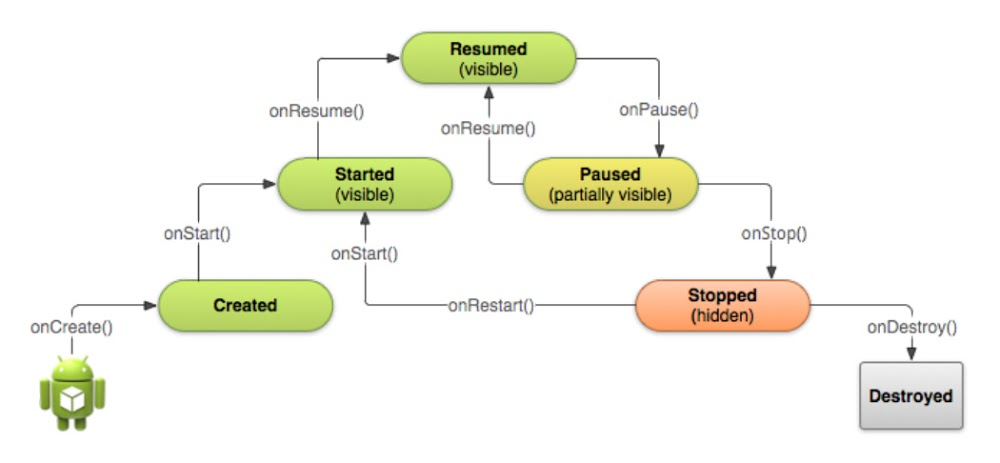
\includegraphics[width=0.8\columnwidth]{Figures/2/lifecycle}
		\caption{วัฏจักรของแอคทิวิตี้บนระบบปฏิบัติการแอนดรอยด์}{ที่มา : https://www.dev2qa.com/android-activity-lifecycle-example/}
		\label{Fig:lifecycle}
	\end{figure}

	จากรูปที่ \ref{Fig:lifecycle} แสดงวัฏจักรของแอคทิวิตี้ในรูปแบบโครงสร้างพีระมิดโดยแสดงให้เห็นว่า Method ที่เรียกใช้
	งานอัตโมัติ (Callback Method) ได้แก่ onCreate(), onStart(), onResume() และ onRestart() จะขยับแอคทิวิตี้ขึ้นไปด้านบนสุดที่ Resumed Method
	และมี Method ได้แก่ onPause(), onStop() และ onDestroy() ที่จะขยับแอคทิวิตี้ลงมาด้านล่าง แอคทิวิตี้ยังสามารถกลับไปทำงานที่ตำแหน่ง Resumed Method จากตำแหน่ง Paused และ Stopped ได้อีกด้วย
	
	ในบางครั้งไม่จำเป็นต้องเรียกใช้งาน Callback Method ทั้งหมดเสมอไปขึ้นกับความซับซ้อนของแอคทิวิตี้ อย่างไรก็ตามเป็นสิ่งสำคัญที่นักพัฒนาควรทำความเข้าใจแต่ละ Method เพื่อให้มั่นใจได้ว่าแอปพลิเคชันของที่ได้พัฒนาตอบสนองเป็นไปตามที่ผู้ใช้คาดหวัง ดังนั้น ในการใช้งาน Callback Method
	ที่ถูกวิธีก็จะช่วยให้แอปพลิเคชันทำงานได้เป็นอย่างดี ดังนี้
	\begin{itemize}
		\item ไม่หยุดการทำงานหรือค้าง กรณีมีสายโทรเข้าหรือมีการสลับไปใช้งานแอปพลิเคชันอื่น 
		\item ไม่ใช้ทรัพยากรที่มีค่าของระบบอย่างสูญเปล่า ถ้าไม่มีการใช้งานแอคทิวิตี้ใดๆ 
		\item ไม่กระทบต่อกระบวนการในขั้นตอนการใช้งานของผู้ใช้กรณีออกจากแอปพลิเคชันแล้วกลับเข้ามาใช้งานอีกครั้ง 
		\item ไม่หยุดการทำงานหรือระบบค้างที่กระทบการใช้งานของผู้ใช้กรณีมีการหมุนหน้าจอแนวนอนและแนวตั้งสลับกัน
	\end{itemize}
	
	เหตุการณ์ที่แอคทิวิตี้มีการเปลี่ยน Method ต่าง ๆ ตามแสดงในรูปที่  \ref{Fig:lifecycle}
	แต่มีอยู่ 3 Method เท่านั้นที่แอคทิวิตี้จะยังคงอยู่คงที่ในช่วงเวลาระยะเวลาหนึ่งไม่เปลี่ยนไป Method อื่นในทันที ได้แก่
		\begin{itemize}
		\item Resumed (แสดงอยู่ ทำงานอยู่) ใน Method นี้แอคทิวิตี้จะแสดงอยู่ด้านหน้าสุดและผู้ใช้กำลังใช้งานอยู่ บ่อยครั้งจะเรียกว่า Running Method
		\item Paused (แสดงหน้าจอบางส่วน ไม่ถูกบังสนิท) ใน Method นี้แอคทิวิตี้จะถูกบดบังด้วยแอคทิวิตี้อื่น เช่น แอคทิวิตี้อื่นที่อยู่ด้านหน้าสุดที่แสดงในลักษณะกึ่งโปรงใสหรือไม่ได้แสดงแบบเต็มหน้าจอ  แอคทิวิตี้ในสถานะนี้จะไม่สามารถรับค่าจากผู้ใช้และทำงานคำสั่งใด ๆ ได้
		\item Stopped (แสดงหน้าจอแบบ Background ผู้ใช้มองไม่เห็น) ใน Method นี้ แอคทิวิตี้จะถูกบดบังอย่างสมบูรณ์และผู้ใช้มองไม่เห็นโดยจะถูกย้ายไปอยู่ด้านหลังในขณะที่อยู่ใน Method นี้
		ค่า Activity Instance และตัวแปรทั้งหมดจะยังคงอยู่แต่จะไม่สามารถถูกเรียกมาใช้งานจากโค้ดใด ๆ ได้
		\end{itemize}

		ในขณะที่ Method อื่น เช่น Created และ Started จะแสดงชั่วคราวแล้วระบบก็จะเปลี่ยนไป Method อื่นในทันทีที่ Method ถูกเรียกใช้งานอัตโนมัติ นั่นคือ หลังจากที่ระบบเรียกใช้งาน onCreate() แล้วก็จะเรียกใช้งาน onStart() ทันทีและสุดท้ายตามด้วย onResumne()  ซึ่งก็จะเข้าสู่ Resumed Method ทั้งหมดก็คือวัฏจักรแอคทิวิตี้เบื้องต้น

	
% IOS 

	\subsection{ความรู้พื้นฐานระบบปฏิบัติการ iOS}
	ระบบปฏิบัติการไอโอเอส (iOS) \cite{iosref} มีชื่อเดิมว่า iPhone OS เริ่มต้นด้วยการเปิดตัวของ iPhone เมื่อวันที่ 29 มิถุนายน 2550 ระบบปฏิบัติการไอโอเอส (iOS) เป็นระบบปฏิบัติการสำหรับสมาร์ทโฟน (Smartphone) ของแอปเปิล โดยเริ่มต้นพัฒนาสำหรับใช้ในโทรศัพท์ iPhone และได้พัฒนาต่อใช้สำหรับ iPot Touch และiPad โดยระบบปฏิบัติการนี้สามารถเชื่อมต่อไปยังแอ็ปสตอร์สำหรับการเข้าถึงถึงแอพพลิเคชั่น(Application) มากกว่า 300,000 ตัว ซึ่งมีการดาวน์โหลดไปมากกว่าห้าพันล้านครั้ง แอปเปิลได้มีการพัฒนาปรับปรุงสำหรับ iPhone, iPad และ iPod Touch ผ่านทางระบบ iTunes คือโปรแกรมฟรี สำหรับ Mac และ PC ใช้ดูหนังฟังเพลงบนคอมพิวเตอร์ รวมทั้งจัดระเบียบและ sync ทุกๆอย่าง และเป็นร้านขายความบันเทิงบนคอมพิวเตอร์, บน iPod touch, iPhone และ iPad ที่มีทุกๆอย่างสำหรับคุณ ในทุกที่และทุกเวลา พัฒนาระบบรักษาความปลอดภัยให้มีความเป็นเลิศ ซึ่งนี้คือข้อได้เปรียบ เมื่อเทียบกับคู่แข่ง	

	\subsubsection{เวอร์ชันของ iOS} 
	iOS 1 (iPhone OS)

	สำหรับ iOS 1 ถูกเปิดตัวครั้งแรกที่งาน Macworld วันที่ 9 มกราคม 2007 พร้อมกับ iPhone รุ่นแรก และหลังจากนั้นก็ออกวางจำหน่ายพร้อม iPhone วันที่ 29 มิถุนายน 2007 สำหรับ iOS 1 มาพร้อมฟีเจอร์เด่น ๆ เช่น ระบบสัมผัสแบบมัลติทัช, voicemail, ท่องเว็บผ่าน Safari และดู YouTube แต่ iOS 1 ไม่ได้ฟรีสำหรับผู้ใช้งาน iPod touch จะต้องจ่ายเงิน 19.99 เหรียญ หรือประมาณ 690 บาท เพื่ออัปเดตเป็น iOS 1

	\begin{figure}[H]
		\centering
		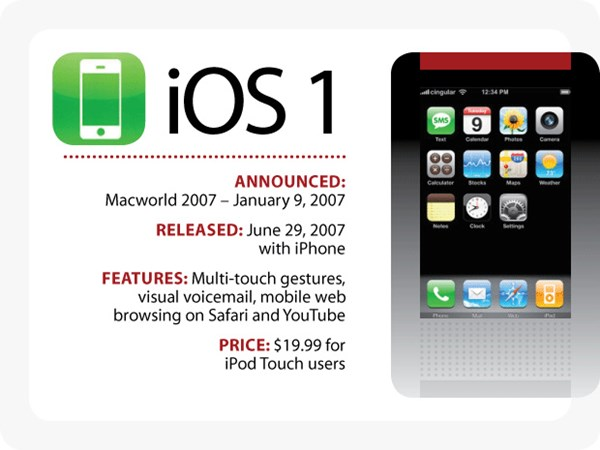
\includegraphics[width=0.8\columnwidth]{Figures/2/iOS/iOS1}
		\caption{iOS 1}{ที่มา : https://mobile.kapook.com/view5432.html}
		\label{Fig:iosversion1}
	\end{figure}

	iOS 2 (iPhone OS 2.0)

	เปิดตัวครั้งแรกที่งาน WWDC 2008 (วันที่ 9 มิถุนายน 2008) และหลังจากนั้นก็ออกวางจำหน่ายพร้อม iPhone 3G วันที่ 11 กรกฎาคม 2008 โดยมีฟีเจอร์เด่น ๆ เช่น App Store, แผนที่พร้อม GPS และระบบแจ้งเตือนอีเมล และเหมือนเช่นเคยผู้ใช้ iPhone สามารถอัปเดตได้ฟรี แต่ผู้ใช้ iPod touch จะต้องจ่ายเงิน 9.95 เหรียญ หรือประมาณ 390 บาท เพื่ออัปเดต iOS 2.x

	\begin{figure}[H]
		\centering
		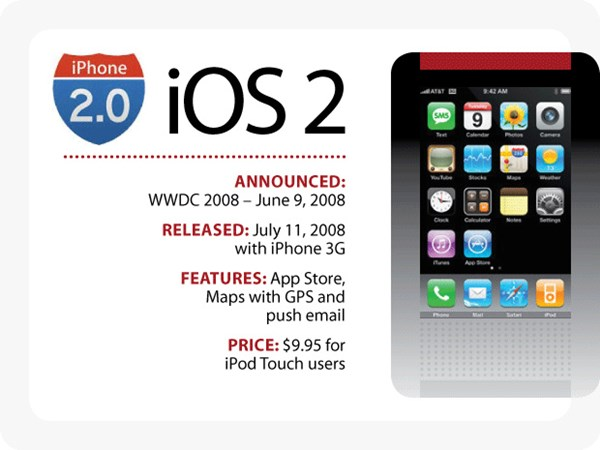
\includegraphics[width=0.8\columnwidth]{Figures/2/iOS/iOS2}
		\caption{iOS 2}{ที่มา : https://mobile.kapook.com/view5432.html}
		\label{Fig:iosversion2}
	\end{figure}

	iOS 3 (iPhone OS 3.0)

	เปิดตัวครั้งแรกที่งาน WWDC 2009 (วันที่ 8 มิถุนายน 2009) และหลังจากนั้นก็ออกวางจำหน่ายพร้อม iPhone 3GS วันที่ 19 มิถุนายน 2009 สำหรับเวอร์ชั่นนี้มาพร้อมฟีเจอร์เด่น ๆ อย่าง Voice Control, สามารถคัดลอกและวางข้อความ และส่ง MMS ได้ เหมือนเช่นเคยผู้ใช้ iPhone สามารถอัปเดตได้ฟรี แต่ผู้ใช้ iPod touch จะต้องจ่ายเงิน 9.95 เหรียญ หรือประมาณ 390 บาท เพื่ออัปเดต iOS 3.0 - 3.1 และ 4.95 เหรียญ หรือประมาณ 169 บาท สำหรับอัปเดต iOS 3.2

	\begin{figure}[H]
		\centering
		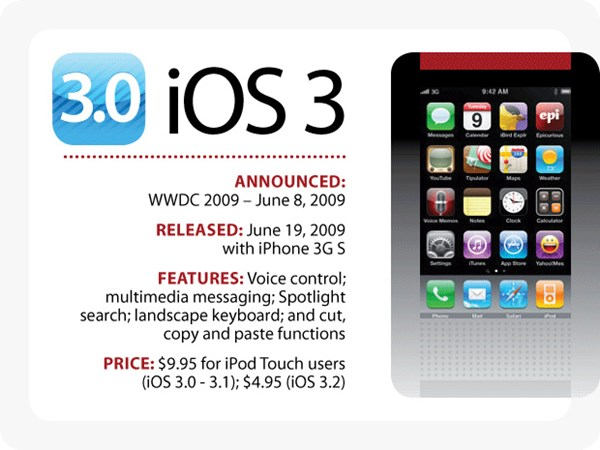
\includegraphics[width=0.8\columnwidth]{Figures/2/iOS/iOS3}
		\caption{iOS 3}{ที่มา : https://mobile.kapook.com/view5432.html}
		\label{Fig:iosversion3}
	\end{figure}

	iOS 4 

	ถือว่าเป็นระบบปฏิบัติการรุ่นแรกของแอปเปิล ที่เปลี่ยนชื่อเรียกจาก iPhone OS มาเป็น iOS โดย iOS 4 เปิดตัวครั้งแรกที่งาน WWDC 2010 (วันที่ 7 มิถุนายน 2010) หลังจากนั้นก็ออกวางจำหน่ายพร้อม iPhone 4 วันที่ 21 มิถุนายน 2010 และมีฟีเจอร์ใหม่ ๆ ที่น่าสนใจมากมาย เช่น Multitasking, โฟลเดอร์, FaceTime, iBook และ iOS 4.2.1 เป็นรุ่นแรกรองรับการใช้งานบน iPad มาถึงเวอร์ชั่นนี้ทุกอุปกรณ์ iOS ของแอปเปิล สามารถอัปเดตได้ฟรี

	\begin{figure}[H]
		\centering
		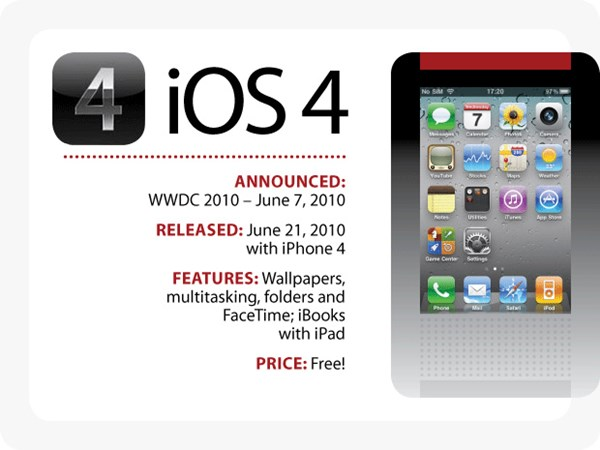
\includegraphics[width=0.8\columnwidth]{Figures/2/iOS/iOS4}
		\caption{iOS 4}{ที่มา : https://mobile.kapook.com/view5432.html}
		\label{Fig:iosversion4}
	\end{figure}

	iOS 5 

	เปิดตัวพร้อม iPhone 4S ที่งาน WWDC 2011 (วันที่ 6 มิถุนายน 2011) และหลังจากนั้นก็ออกวางจำหน่ายพร้อม iPhone 4S วันที่ 12 ตุลาคม 2011 มาพร้อมฟีเจอร์ใหม่ที่น่าสนใจหลายอย่าง เช่น Siri, iCloud, Notification Center, iMessage, Reminders และ Newsstand เป็นต้น

	\begin{figure}[H]
		\centering
		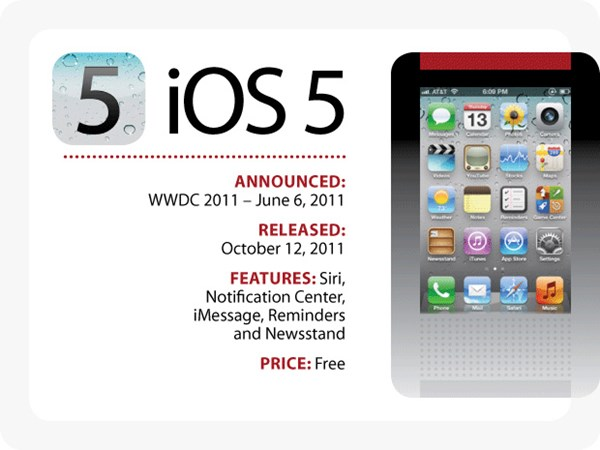
\includegraphics[width=0.8\columnwidth]{Figures/2/iOS/iOS5}
		\caption{iOS 5}{ที่มา : https://mobile.kapook.com/view5432.html}
		\label{Fig:iosversion5}
	\end{figure}

	iOS 6 

	เปิดตัวพร้อม iPhone 5 และ iPad mini ที่งาน WWDC 2012 (วันที่ 11 มิถุนายน 2012) และออกวางจำหน่ายพร้อม iPhone 5 วันที่ 19 กันยายน 2012 สำหรับฟีเจอร์ใหม่ที่มาพร้อม iOS 6 เช่น การเปลี่ยนไปใช้ระบบแผนที่ของแอปเปิลเอง, สามารถ Facetime ผ่านระบบเซลลูลาร์, ถ่ายภาพแบบพาโนรามา, คีย์บอร์ดภาษาไทยแบบ 4 แถว, Passbook, อินทิเกรท Facebook, รองรับ LTE และแอปฯ นาฬิกาสำหรับ iPad

	\begin{figure}[H]
		\centering
		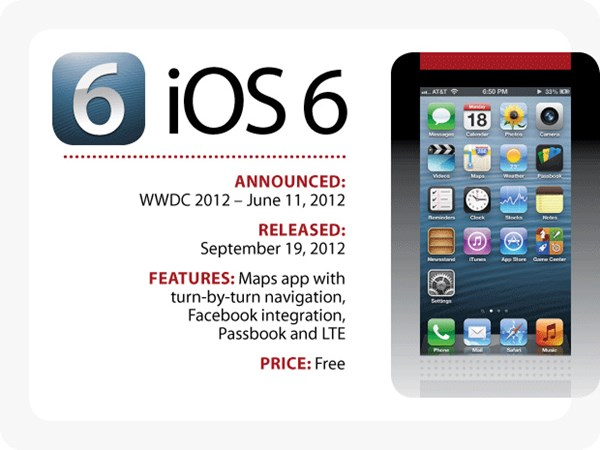
\includegraphics[width=0.8\columnwidth]{Figures/2/iOS/iOS6}
		\caption{iOS 6}{ที่มา : https://mobile.kapook.com/view5432.html}
		\label{Fig:iosversion6}
	\end{figure}

	iOS 7 

	อีกก้าวสำคัญของแอปเปิล ที่มีการยกเครื่องเปลี่ยนดีไซน์ของ iOS ใหม่ทั้งหมด เปิดตัวครั้งแรกที่งาน WWDC 2013 (วันที่ 10 มิถุนายน 2013) และปล่อยให้อัปเดตวันที่ 18 กันยายน 2013 โดยผู้ที่รับหน้าที่ดูแลการปรับโฉม iOS 7 ครั้งนี้ ก็คือ Jonathan Ive เปลี่ยนมาใช้ดีไซน์แบบ Flat Design, ไอคอนใหม่ทั้งหมด, มี Control Center, AirDrop, Photos, iTunes Radio และ CarPlay

	\begin{figure}[H]
		\centering
		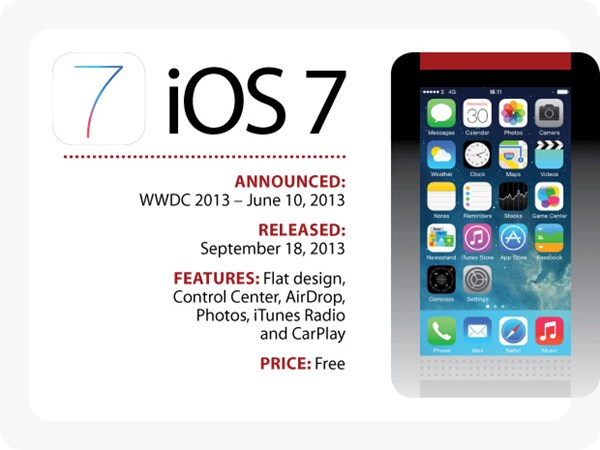
\includegraphics[width=0.8\columnwidth]{Figures/2/iOS/iOS7}
		\caption{iOS 7}{ที่มา : https://mobile.kapook.com/view5432.html}
		\label{Fig:iosversion7}
	\end{figure}

	iOS 8 

	สำหรับ iOS 8 เปิดตัวครั้งแรกที่งาน WWDC 2014 (วันที่ 2 มิถุนายน 2014) และปล่อยให้อัปเดตวันที่ 17 กันยายน 2014 พร้อมการเปิดตัว iPhone 6, 6 Plus และ iPad Air 2 โดยหน้าตาต่าง ๆ ของ iOS 8 ยังคงเหมือนกับ iOS 7 แต่ปรับปรุงประสิทธิภาพการทำงานให้ดีขึ้นกว่าเดิม รวมถึงเพิ่มฟีเจอร์การใช้งานต่าง ๆ เข้ามาอีกอย่างมากมาย เช่น iCloud Drive, Apple Pay, Apple Music, QuickType, Family Sharing และแอปฯ Health เป็นต้น

	\begin{figure}[H]
		\centering
		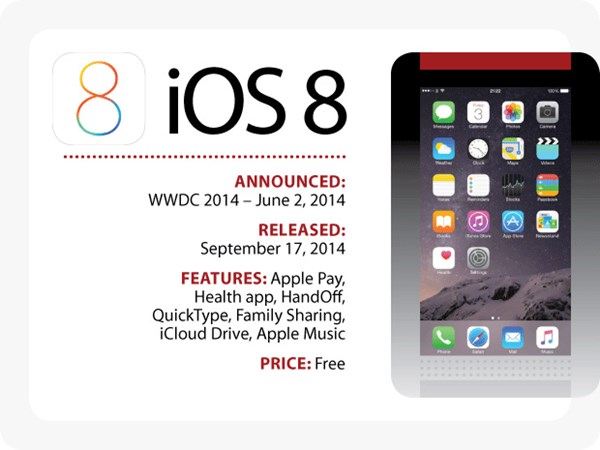
\includegraphics[width=0.8\columnwidth]{Figures/2/iOS/iOS8}
		\caption{iOS 8}{ที่มา : https://mobile.kapook.com/view5432.html}
		\label{Fig:iosversion8}
	\end{figure}

	iOS 9 

	เปิดตัวครั้งแรกที่งาน WWDC 2015 (วันที่ 8 มิถุนายน 2015) และปล่อยให้อัปเดตวันที่ 16 กันยายน 2015 สำหรับเวอร์ชั่นนี้เน้นปรับปรุงเพิ่มประสิทธิภาพการใช้งานให้ดีขึ้นกว่าเดิม รวมถึงเปลี่ยนแปลงและเพิ่มฟีเจอร์ใหม่ที่ช่วยให้ผู้ใช้สะดวกสบายมากขึ้น โดยฟีเจอร์หลาย ๆ อย่างเรียนรู้จากพฤติกรรมผู้ใช้งาน เพื่อตอบสนองสิ่งที่ผู้ใช้งานต้องการมากที่สุด โดยฟีเจอร์ใหม่ที่มาพร้อม iOS 9 เช่น Siri มีความแม่นยำและทำงานได้รวดเร็วกว่าเดิม, รองรับการใช้งาน 2 หน้าจอสำหรับ iPad, เพิ่มแอปฯ News, ปรับปรุงแอปฯ Note, Spotlight ให้สามารถค้นหาสิ่งต่าง ๆ ได้มากขึ้น

	\begin{figure}[H]
		\centering
		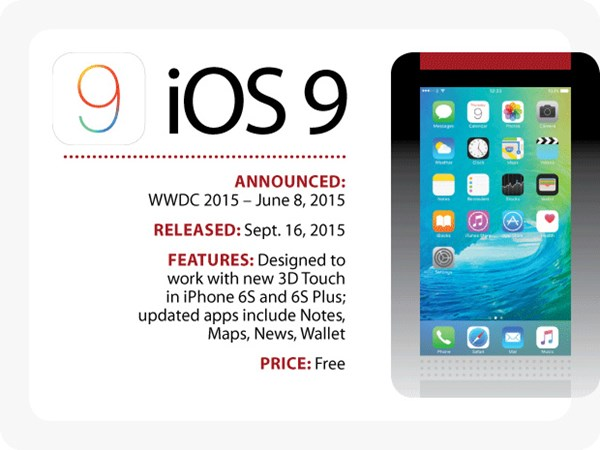
\includegraphics[width=0.8\columnwidth]{Figures/2/iOS/iOS9}
		\caption{iOS 9}{ที่มา : https://mobile.kapook.com/view5432.html}
		\label{Fig:iosversion9}
	\end{figure}

	iOS 10 

	เปิดตัวครั้งแรกที่งาน WWDC 2016 (วันที่ 13 มิถุนายน 2016) และปล่อยให้อัปเดตวันที่ 13 กันยายน 2016 แอปเปิลบอกว่า iOS 10 มาพร้อมการปรับปรุงครั้งใหญ่ ภายในงานได้พูดถึง 10 ฟีเจอร์หลัก ๆ ที่มีการเปลี่ยนแปลงหลาย ๆ อย่าง เช่น อินเทอร์เฟซมีการปรับเปลี่ยนใหม่ให้ดูสวยงามขึ้นกว่าเดิม, ระบบแจ้งเตือนแบบใหม่, 3D Touch ที่ใช้งานได้หลากหลายขึ้น, รีดีไซน์แอปฯ Apple Maps, Apple Music และ News เป็นต้น

	\begin{figure}[H]
		\centering
		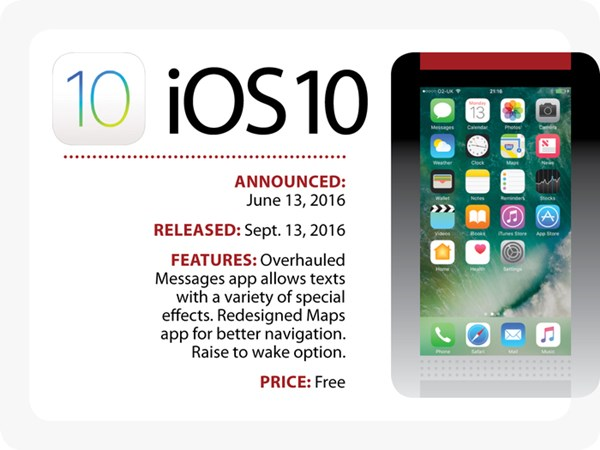
\includegraphics[width=0.8\columnwidth]{Figures/2/iOS/iOS10}
		\caption{iOS 10}{ที่มา : https://mobile.kapook.com/view5432.html}
		\label{Fig:iosversion10}
	\end{figure}

	iOS 11 

	เปิดตัวครั้งแรกที่งาน WWDC 2017 (วันที่ 5 มิถุนายน 2017) และปล่อยให้อัปเดตวันที่ 19 กันยายน 2017 สำหรับเวอร์ชั่นนี้แอปเปิลได้ให้คำนิยามไว้ว่า "เป็นก้าวใหญ่สำหรับ iPhone ก้าวกระโดดสำหรับ iPad" โดยเน้นการปรับปรุงเพิ่มความสามารถรอบด้าน ตอบโจทย์การใช้งานให้ดีขึ้นกว่าเดิม โดยของใหม่ที่มาพร้อม iOS 11 ที่น่าสนใจ เช่น Siri สามารถแปลภาษาได้, ปรับปรุง Control Center ใหม่, Apple Pay รองรับการโอนเงินได้, เพิ่ม API สำหรับระบบ AR เทคโนโลยีที่ผสมผสานระหว่างความเป็นจริงและโลกเสมือน รวมถึงฟีเจอร์ป้องกันการใช้โทรศัพท์ขณะขับรถ

	\begin{figure}[H]
		\centering
		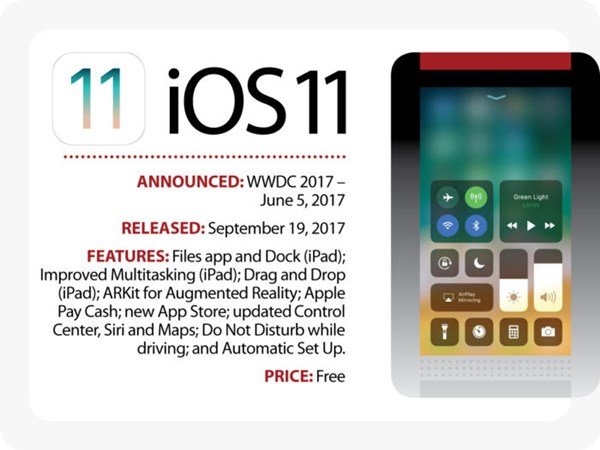
\includegraphics[width=0.8\columnwidth]{Figures/2/iOS/iOS11}
		\caption{iOS 11}{ที่มา : https://mobile.kapook.com/view5432.html}
		\label{Fig:iosversion11}
	\end{figure}
	
	iOS 12 

	เปิดตัวครั้งแรกที่งาน WWDC 2018 (วันที่ 4 มิถุนายน 2018) และจะปล่อยให้อัปเดตในช่วงเดือนกันยายน 2018 หรือหลังจากเปิดตัว iPhone รุ่นใหม่ไปแล้ว สำหรับ iOS 12 ยังคงพัฒนาอย่างต่อเนื่อง โดยออกแบบมาเพื่อทำให้การทำงานประจำวันดำเนินไปอย่างรวดเร็วและตอบสนองฉับไวขึ้น iOS 12 จะเปลี่ยนวิธีการที่ผู้ใช้ iOS มองเห็นโลกโดยใช้ AR ทำให้การสื่อสารมีความสนุกสนานและสื่ออารมณ์ด้วย Memoji, Group FaceTime และ Screen Time ช่วยทำความเข้าใจและจัดการกับเวลาการใช้งานอุปกรณ์ iOS ลดการติดมือถือ นอกจากนี้ยัง iOS 12 เปิดตัว Siri Shortcuts ซึ่งจะทำให้ Siri สามารถทำงานร่วมกับแอปฯ ใดก็ได้

	\begin{figure}[H]
		\centering
		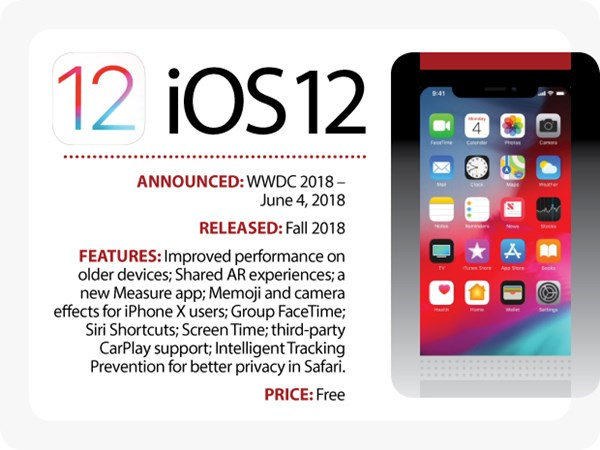
\includegraphics[width=0.8\columnwidth]{Figures/2/iOS/iOS12}
		\caption{iOS 12}{ที่มา : https://mobile.kapook.com/view5432.html}
		\label{Fig:iosversion12}
	\end{figure}

% Ionic Framework

	 \subsection{ความรู้พื้นฐาน Ionic Framework}
	 Ionic Framework \cite{ionicref} คือเครื่องมือในการสร้าง Mobile Application เป็นเครื่องมือสร้างแอปมือถือที่สามารถสร้างทีเดียว สามารถใช้งานได้บนระบบปฏิบัติการ 
	 iOS, Android และ Windows ซึ่งก็จะใช้งานร่วมกับ Framework ตัวอื่น ๆ ได้ คือ Angular และ Apache Cordova 
	 ในตอนสุดท้าย เพื่อให้ทั้งแอปที่เขียนมาใช้ได้กับทุกระบบปฏิบัติการ

		\subsubsection{เทคโนโลยีที่ใช้ในการพัฒนา Ionic Framework} 
		Ionic Framework พัฒนา Frontend ด้วยภาษา HTML , CSS , JavaScript และถูก Build เป็น Application ด้วย Cordova
		\begin{itemize}
		\item HTML5  คือ คือ ภาษามาร์กอัป ที่ใช้สำหรับเขียน website ซึ่ง HTML5 นี้เป็นภาษาที่ถูกพัฒนาต่อมาจากภาษา HTML และพัฒนาขึ้นมาโดย WHATWG (The Web Hypertext Application Technology Working Group) โดยได้มีการปรับเพิ่ม Feature หลายๆอย่างเข้ามาเพื่อให้ผู้พัฒนาสามารถใช้งานได้ง่ายมากยิ่งขึ้น
		\item CSS3  คือ สไตล์ชีท เป็นภาษาที่ใช้เป็นส่วนของการจัดรูปแบบการแสดงผลของ HTML พูดง่ายๆ คือทำให้การแสดงผลของ HTML ให้สวยงาม
		\item AngularJs คือ JavaScript Framework  รูปแบบหนึ่งที่พัฒนามาจาก Google หน้าที่ของมันคือเป็น engine ที่ใช้ควบคุมในส่วน front end ของเว็บได้เป็นอย่างดีมีการทำงานแบบ Model View Controller (MVC)
		\end{itemize}
		\begin{figure}[H]
			\centering
			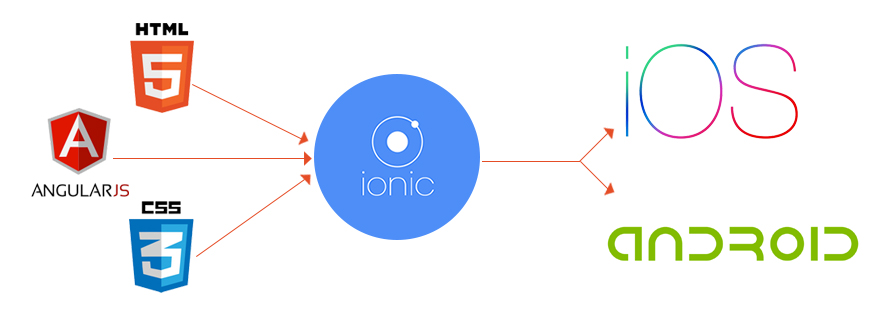
\includegraphics[width=0.8\columnwidth]{Figures/2/ionic1}
			\caption{การทำงานของ Ionic Framework}{ที่มา : http://blog.prscreative.com/what-is-ionic/}
			\label{Fig:ionic}
		\end{figure}

		\subsubsection{การทำงานของ Cordova Application}
		การทำงานของ Hybrid Mobile App คือในช่อง Web App จะมี HTML, CSS, Javascript และไฟล์ภาพ เสียงต่างๆ (Resource) แล้วทำงานผ่าน Web View ที่ PhoneGap จัดเตรียมให้ หากต้องการเข้าถึงส่วนอื่นๆก็เรียกใช้ Plug-in หรือจะพัฒนา Custom Plug-in ขึ้นมาใช้เองได้ ดังรูปที่ \ref{Fig:ionic1}
		
		\begin{figure}[H]
			\centering
			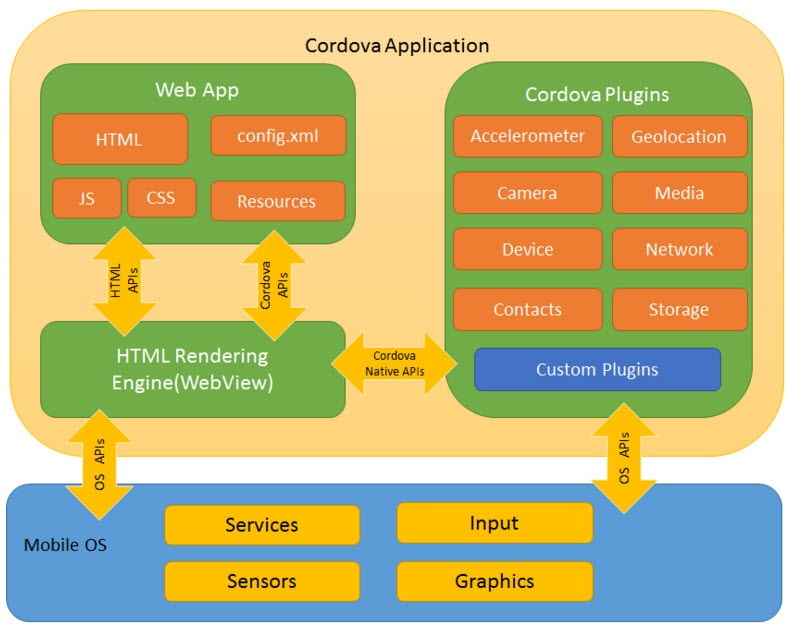
\includegraphics[width=0.8\columnwidth]{Figures/2/ionic2}
			\caption{Cordova Application}{ที่มา : http://blog.prscreative.com/what-is-ionic/}
			\label{Fig:ionic1}
		\end{figure}

		โดย Cordova มีหน้าที่ห่อหุ้มแอปพลิเคชันไว้ และทำหน้าที่ติดต่อกับ Hardware ของ Mobile เป็นหลักเพราะมี API ติดต่อกับ Hardware โดยตรง เช่น Camera, Contacts, Media, Network
		
		\subsubsection{ความแตกต่างระหว่าง PhoneGap/Cordova} 
		PhoneGap และ Cordova มีลักษณะคล้ายกัน เนื่องจากมันเกือบจะเหมือนกัน ต่างกันเพียงเรื่องของลิขสิทธิ์ และการนำไปใช้งาน

		\begin{enumerate}[label=\arabic*)]
		\item PhoneGap : ในยุคแรกถูกพัฒนาโดย Nitobi เปิดให้ใช้งานแบบ Open Source ซึ่งได้รับความนิยมในการนำมาใช้เป็นเทคโนโลยี Hybrid ซึ่งต่อมาถูกซื้อโดยบริษัท Adobe เพื่อนำมาเสริมทัพให้กับโปรแกรม Adobe Dreamweaver เพื่อให้สั่ง Build app จากโปรแกรม Dreamweaver ให้ลองรับหลาย Platform ได้ แต่มีค่าลิขสิทธิ์โปรแกรม
		\item Cordova : เกิดขึ้นจากการตกลงกันระหว่าง Adobe และ Nitobi ด้วยแนวคิดที่อยากให้ PhoneGap เป็น Open Source ต่อไป จึงได้มีการตกลงกันให้นำโค๊ดของ PhoneGap ไปตั้งเป็นชื่อใหม่ นั่นก็คือ Cordova เพื่อมอบให้ Apache Foundation ไปดูแลถูกนำไปใช้ในโครงการ Hybrid mobile application หลายโครงการ เช่น AppGyver, Ionic framework
		\end{enumerate}

		\subsubsection{ เริ่มต้นการใช้งาน}
		การเริ่มต้นใช้งาน Ionic Framework สามารถศึกษาการติดตั้งได้ที่ https://ionicframework.com/docs/v3/intro/installation/ ซี่งเริ่มต้นเราจะต้องทำการติดตั้ง Cordova CLI และ Ionic CLIผ่าน npm ก่อน
		\begin{figure}[H]
			{\setstretch{1.0}\begin{lstlisting}
$ npm install -g cordova 
# ติดตั้ง Cordova CLI
$ npm install -g ionic 
# ติดตั้ง Ionic CLI
$ ionic start ชื่อโปรเจค
# สร้างโปรเจคไอโอนิกมีลักษณะธีมเริ่มต้นเป็น Blank
$ cd ชื่อโปรเจค
# เข้าไปในโปรเจคที่เราสร้าง
$ ionic serve
# รันไอโอนิกแบบ localhost:8000
				\end{lstlisting}}
			\centering
			\caption{แสดงการติดตั้ง cli}
			\label{Fig:moment}
		\end{figure}


% Firebase

\subsection{Firebase}
	Firebase \cite{firebase} คือ บริการ Backend และ แพลตฟอร์ม ครบวงจรสำหรับนักพัฒนาแอปพลิเคชัน และโปรแกรมประยุกต์บนเว็บแพลตฟอร์มที่มีเครื่องมือและโครงสร้างพื้นฐานที่ได้รับการออกแบบมาเพื่อช่วยให้นักพัฒนาสามารถสร้างแอปพลิเคชันพลิเคที่มีคุณภาพสูง Firebase (ไฟร์เบส) ถูกสร้างขึ้นจากคุณสมบัติเสริมว่านักพัฒนาสามารถผสมและจับคู่เพื่อให้พอดีกับความต้องการของตน บริษัท ก่อตั้งขึ้นในปี 2011 โดยแอนดรูลีและเจมส์ เทมปลิน สินค้าเริ่มต้น Firebase) เป็นฐานข้อมูลเรียลไทม์ซึ่งมี API ที่ช่วยให้นักพัฒนาในการจัดเก็บและซิงค์ข้อมูล ดังรูป \ref{Fig:class1}
	
	Google Firebase 2.0 มีการพัฒนาจากบริการ Backend เก็บข้อมูลอย่างเดียว มาเป็น แพลตฟอร์มครบวงจรสำหรับนักพัฒนาแอปพลิเคชัน (รองรับ iOS, Android, Web) และรองรับบริการทุกอย่างที่นักพัฒนาแอปต้องการใช้งาน
	
	\begin{figure}[H]
		\centering
		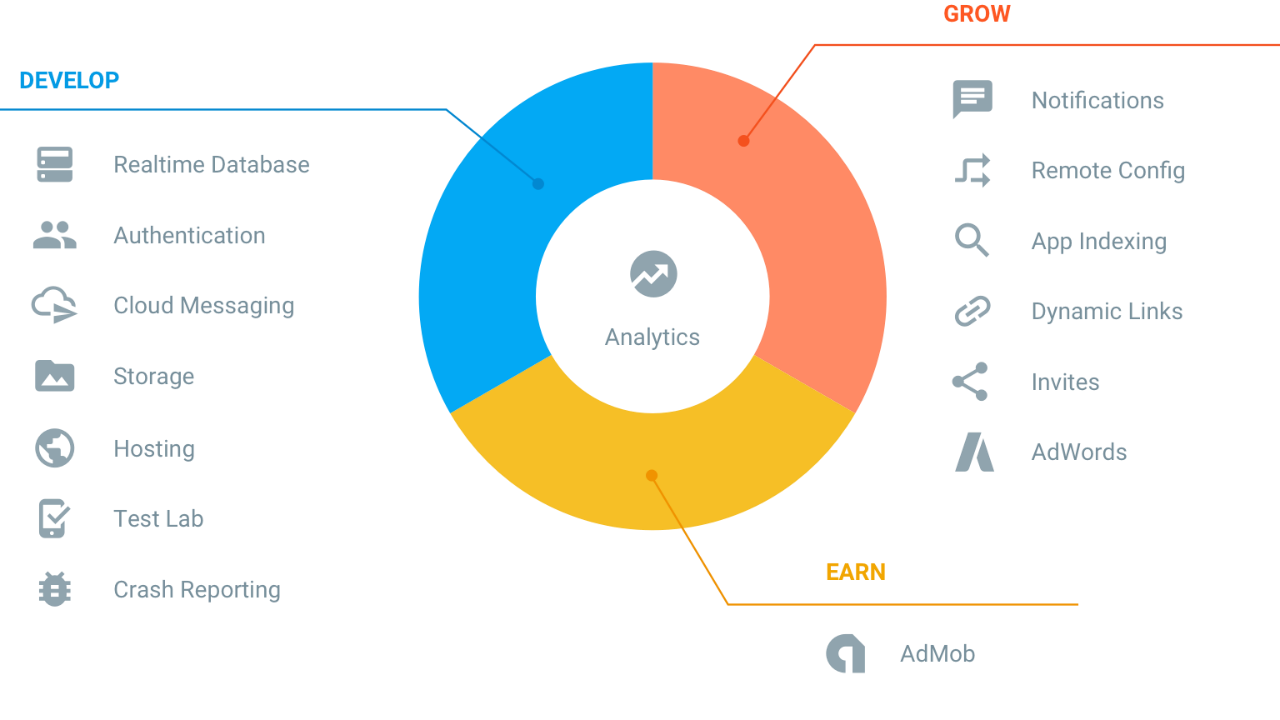
\includegraphics[width=\columnwidth]{Figures/2/firebase}
		\caption{Firebase 2.0}{ที่มา : www.mindphp/คู่มือ/73-คืออะไร/3921-what-is-firebase-backend.html}
		\label{Fig:class1}
	\end{figure}

\subsubsection{บริการหลักของไฟร์เบส} 

\begin{itemize}
	\item Realtime Database จัดเก็บและซิงค์ข้อมูลระหว่างผู้ใช้และอุปกรณ์ต่างๆแบบเรียลไทม์โดยใช้ฐานข้อมูล NoSQL ที่โฮสต์บนระบบคลาวด์ ซิงค์ข้อมูลที่อัปเดตระหว่างอุปกรณ์ที่เชื่อมต่อเป็นมิลลิวินาทีและข้อมูลจะยังคงมีอยู่ถ้าแอพพลิเคชันออฟไลน์
	\item Authentication จัดการบัญชีผู้ใช้ด้วย Firebase Auth ซึ่งใช้งานง่ายและปลอดภัยมีวิธีการหลายในการสร้างบัญชีผู้ใช้และตรวจสอบความถูกต้อง ได้แก่ อีเมล/รหัสผ่าน, ผู้ให้บริการบุคคลที่สามเช่น Google หรือ Facebook 
	\item Cloud Storage จัดเก็บภาพเสียงวิดีโอหรือเนื้อหาอื่น ๆ เช่น รูปภาพโปรไฟล์ผู้ใช้ หรือวีดีทัศน์ต่างๆ เป็นต้น ซึ่งมีความปลอดภัยในการอัปโหลดไฟล์และดาวน์โหลดสำหรับแอพพลิเคชัน
	\item Hosting ใช้ในการเผยแพร่เว็บไซต์  โดยเนื้อหาภายในเว็บเป็นเดชบอร์ด รายงานข้อต่างๆ ของผู้ใช้ ซึ่งต้องทำการเข้าสู่ระบบก่อน
	\item Crashlytics เป็นบริการล่าสุดที่กูเกิลได้เข้าควบรวมเข้ามาไว้ในบริการไฟร์เบส สามารถรายงานข้อขัดข้องได้อย่างมีประสิทธิภาพ เปิดใช้งานการวิเคราะห์แบบเรียลไทม์เพื่อช่วยให้เข้าใจสิ่งที่เกิดขึ้นในแอพพลิเคชัน เครื่องมือวิเคราะห์ข้อมูลจะให้ข้อมูลเชิงลึก
	\item Cloud Firestore เป็นบริการในส่วนของ Database ที่ใช้ระบบฐานของข้อมูลแบบ NoSQL ที่เป็นแบบ Document Database และเป็นการนำเอาข้อดีต่างๆของบริการด้านฐานข้อมูลของ Realtime Database มาปรับปรุงพัฒนาต่อและเพิ่มความสามารถขึ้นไปมากขึ้น ซึ่งผู้เขียนจะได้กล่าวถึงในบทถัดไป
\end{itemize}

\subsubsection{การพัฒนา Cloud Firestore} 
การพัฒนา Cloud Firestore แบ่งออกแบบ 5 ขั้นตอน ดังนี้

\begin{enumerate}[label=\arabic*)]
	\item การสร้าง Cloud Firestore เพื่อใช้งานในโครงการ ในขั้นตอนแรกทำการสร้าง Database เพื่อที่จะใช้งาน Cloud Firestore ก่อน โดยใช้บัญชี Gmail ต่อมาเข้าไปที่เว็บ https://firebase.google.com  ดังรูปภาพที่ \ref{Fig:f1}
	\begin{figure}[H]
		\centering
		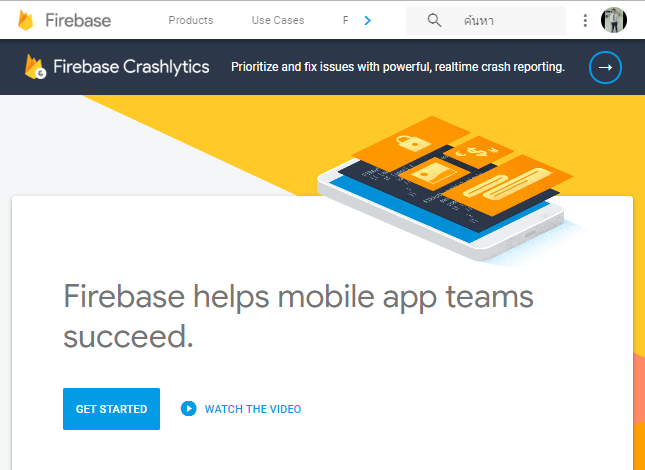
\includegraphics[width=0.7\columnwidth]{Figures/2/f1}
		\caption{เว็บ https://firebase.google.com}{ที่มา :https://medium.com/20scoops-cnx/เข้มข้นกับ-firebase-cloud-firestore-ระบบฐานข้อมูลที่เปิดตัวใหม่ล่าสุดจาก-firsbase-แบบจัดเต็ม-d001e43e2be7 }
		\label{Fig:f1}
	\end{figure}
	\item ติดตั้ง SDKs เพื่อใช้งาน Cloud Firestore
	โดย SDKs ที่ Firebase ได้เตรียมไว้ให้ สามารถดูรายละเอียดได้ที่ https://firebase.google.com/docs/firestore/quickstart
	\item ออกแบบโครงสร้างและการจัดการข้อมูล  
	\begin{itemize}
		\item ระบบฐานข้อมูลของ Cloud Firestore จะเป็น NoSQL แบบ Document ซึ่งจะแตกต่างจากระบบฐานข้อมูลแบบ SQL โดยจะไม่มีตาราง ไม่มีแถว แต่เก็บข้อมูล ภายใน Document จะเก็บแบบ Key-value โดยแต่ละ Document จะถูกเก็บไว้ใน Collection ซึ่งใน Document สามารถมี Subcollection ได้
		\item Collection เป็นการเรียกชื่อแทนของการเก็บหลายๆเอกสารไว้ด้วยกัน เช่น เก็บข้อมูลของ User จำนวนมากไว้ด้วยกัน จึงตั้งชื่อ Collection ว่า Users ซึ่งใน Collection เดียวกันผู้ใช้งานสามารถใส่ข้อมูลที่แตกต่างชนิดกันในแต่ละ Key แต่ละ Document ได้ โดยในแต่ละ Key และ Document จะมีอิสระในการใส่ข้อมูล แต่ควรใส่ข้อมูลในแต่ละ Key ของ Document เป็นประเภทเดียวกันเพราะจะทำให้การค้นหาและการจัดเรียงลำดับของข้อมูลนั้นง่ายขึ้น
		\item Subcollection สามารถสร้าง Subcollection ของ Subcollection ไปได้เรื่อยๆ โดย Cloud Firestore ว่าสามารถซ้อนกันไปได้ 100 ลำดับชั้น
	\end{itemize}
	\item การรับและสอบถามข้อมูล
	การรับและสอบถามข้อมูลจาก Cloud Firestore จะมี 2 วิธี โดยจะสามารถใช้ได้ทั้งการรับข้อมูลและการสอบถามข้อมูล
	\begin{itemize}
		\item การรับข้อมูลเพียงครั้งเดียวจะเป็นการรับข้อมูลเมื่อมีจุดประสงค์ที่จะไม่ต้องการรับรู้การเปลี่ยนแปลงของข้อมูล ซึ่ง ณ ขณะนั้นข้อมูลมีค่าเป็นอะไรก็จะได้ค่านั้นมา หากมีการเปลี่ยนแปลงข้อมูลในภายหลัง ผู้ใช้งานต้องเป็นผู้จัดการรับข้อมูลล่าสุดเอง โดยวิธีการรับข้อมูลเพียงครั้งเดียวจะใช้ Method Get()
		\item การรับข้อมูลแบบ Realtime update จะเป็นการรับข้อมูลเมื่อผู้ใช้งานมีจุดประสงค์ที่จะต้องการรับรู้การเปลี่ยนแปลงของข้อมูล ซึ่ง ณ ขณะที่ข้อมูลเกิดการเปลี่ยนแปลงจะมีการรับข้อมูลที่เกิดการเปลี่ยนแปลงโดยอัตโนมัติ โดยในครั้งแรกที่มีการรับข้อมูลจะสร้าง Initialize Instance และทุกครั้งที่ข้อมูลมีการเปลี่ยนแปลงก็จะส่ง Callback ให้กับ Iistener โดยผ่าน Method onSnapshot()
	\end{itemize}
	\item การป้องกันและความปลอดภัยของข้อมูลข้อมูลใน Cloud Firestore ได้มีการออกแบบให้สามารถกำหนดกฏของความปลอดภัยต่างๆได้ โดยผ่าน Firebase Console  ซึ่งหากใช้ Cloud Firestore ผู้ใช้งานสามารถมาทำเรื่องการป้องกันและรักษาความปลอดภัยของข้อมูลเพียงที่เดียวก็สามารถใช้ได้ทั้งหมดไม่ว่าจะเป็น Web และ Mobile ส่วนฝั่ง Server ก็สามารถใช้ IAM ใน Google Cloud Platform มาจัดการความปลอดภัยสำหรับ Cloud Firestore ได้
\end{enumerate}


% Dialogflow

\subsection{Dialogflow}
Dialogflow คือ platform สำหรับสร้าง chatbot ของ Google ที่ใช้ machine learning ด้าน Natural Language Processing (NLP) มาช่วยในทำความเข้าใจถึงความต้องการ (intent) และสิ่งที่ต้องการ (entity) ในประโยคสนทนาของผู้ใช้งาน และตอบคำถามตามความต้องการของผู้ใช้งาน ตามกฎ หรือ flow ที่ผู้พัฒนาวางเอาไว้ ซึ่ง Dialogflow จะช่วยเพิ่มความยืดหยุ่นของประโยคที่ chatbot รับมา ว่าไม่จำเป็นต้องตรงตามเงื่อนไข แบบ rule based ก็สามารถเข้าใจถึงความต้องการของผู้ใช้งานได้

 \begin{figure}[H]
	\centering
	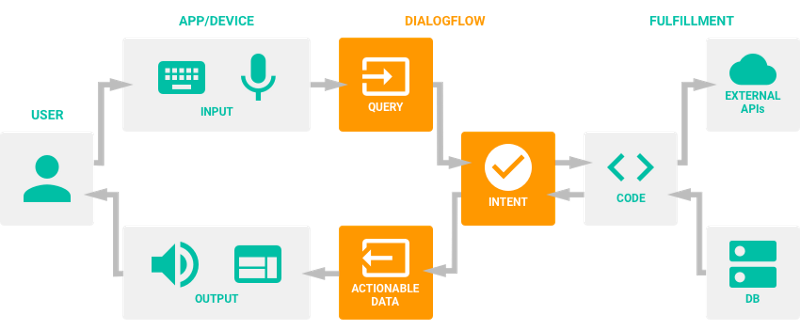
\includegraphics[width=0.9\columnwidth]{Figures/2/chatbot}
	\caption{รูปแบบการส่งข้อมูลผู้ใช้ไปยังแชทบอท}{ที่มา : https://dialogflow.com/docs/agents}
	\label{Fig:dialogflow}
\end{figure}

\subsubsection{เริ่มต้นใช้งาน Dialogflow} 

\begin{enumerate}[label=\arabic*)]
\item ลงทะเบียน/ล๊อกอินเข้า Dialogflow \\
ในการสร้าง Agent เราต้องลงทะเบียนเข้าใช้งานก่อนนะ โดยไปยังหน้าเว็บของ Dialogflow และกดที่ Go Console จากนั้นก็เข้าสู่ขั้นตอนการ Login หรือลงทะเบียน

	\begin{figure}[H]
		\centering
		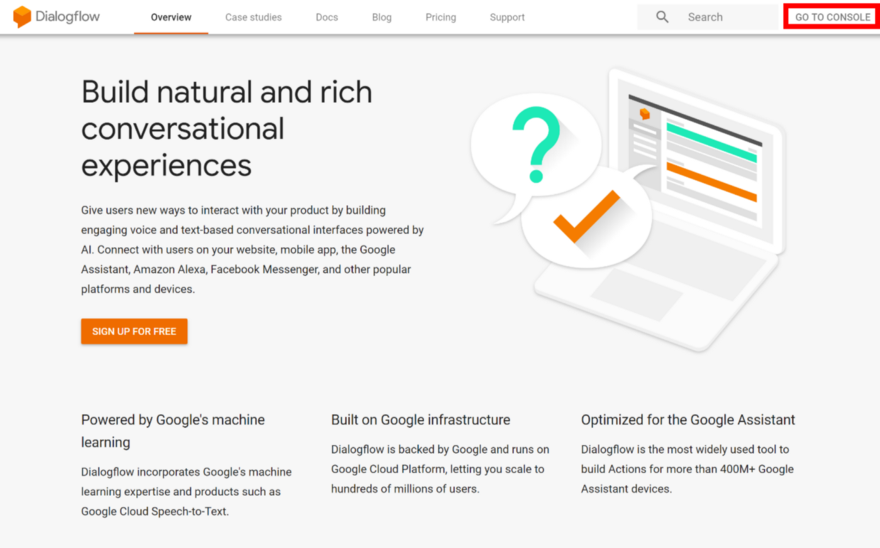
\includegraphics[width=0.9\columnwidth]{Figures/2/dialogflow_1}
		\caption{หน้าหลักของ Dialogflow}
		\label{Fig:dialogflow1}
	\end{figure}

\item สร้าง Agent \\
หลังจาก Login สำเร็จเราก็จะเจอกับ Workplace ในการทำแชทบอทละ ให้ไปที่เมนูด้านซ้าย และเลือก Create Agent ก็จะพบกับหน้าจอสำหรับตั้งค่าแชทบอทของเรา โดยต้องสามารถตั้งชื่อ ภาษา และ Timezone ที่ต้องการ

	\begin{figure}[H]
		\centering
		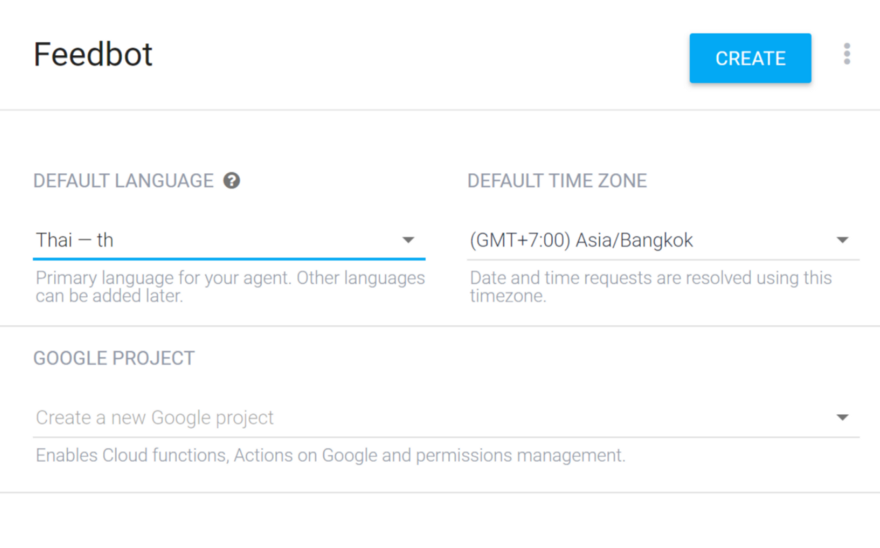
\includegraphics[width=0.9\columnwidth]{Figures/2/dialogflow_2}
		\caption{หน้า Create Agent}
		\label{Fig:dialogflow2}
	\end{figure}

\item สอนบอทให้พูดทักทาย \\
เมื่อสร้างเสร็จแล้วเราจะพบกับ Default Intents มา 2 ตัวก็คือ Default Welcome Intent และ Default Fallback Intent มาให้ ตอนนี้ยังไม่ต้องสนใจมันนะ เพราะเราจะลองสร้าง Intent ใหม่เลยโดยตั้งชื่อว่า Greeting 
ในการสร้างให้กดที่ปุ่ม Create Intent และตั้งชื่อ Intent นี้ว่า Greeting โดยเราตั้งใจจะให้ Intent นี้ โต้ตอบกับผู้ใช้งาน เวลาที่ผู้ใช้ต้องการที่จะทักทายกับแชทบอท ที่เราสร้างขึ้นมา
จากนั้นไปที่ Training phrases หรือแนวประโยคที่เราจะให้แชทบอทเข้าใจว่า ถ้าพูดด้วยประโยคประมาณนี้ แสดงว่าผู้ใช้งานตั้งใจจะสื่อถึง Intent นี้ ถ้าดูจากตัวอย่างจะพบว่ามีการระบุ phrases ไว้ว่า สวัสดี, สวัสดีจ้ะ, สวัสดีจ้า

	\begin{figure}[H]
		\centering
		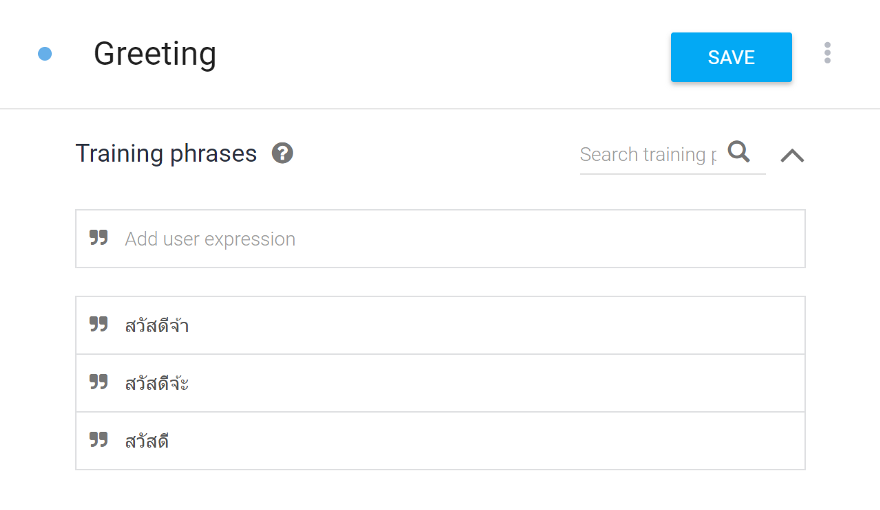
\includegraphics[width=0.9\columnwidth]{Figures/2/dialogflow_3}
		\caption{หน้า Intent ส่วน Training phrases}
		\label{Fig:dialogflow3}
	\end{figure}
	
จากนั้นเราจะลองไปตั้งค่า Responses หรือประโยคที่เราต้องการให้แชทบอทตอบกลับ ในกรณีนี้ที่บอทสามารถจับได้ว่าผู้ใช้งานตั้งใจจะสื่อถึง Intent นี้ สำหรับตัวอย่างจะพบว่า ถ้าผู้ใช้พิมพ์ สวัสดี, สวัสดีจ้ะ, สวัสดีจ้า ตาม Training phrases เราจะให้แชทบอทของเราตอบกลับว่า สวัสดีครับ เป็นยังไงบ้างครับ สบายดีไหม หรือ สวัสดีครับ สบายดีไหมครับ โดยจะสุ่มขึ้นมาว่าจะตอบอันไหน
	
	\begin{figure}[H]
		\centering
		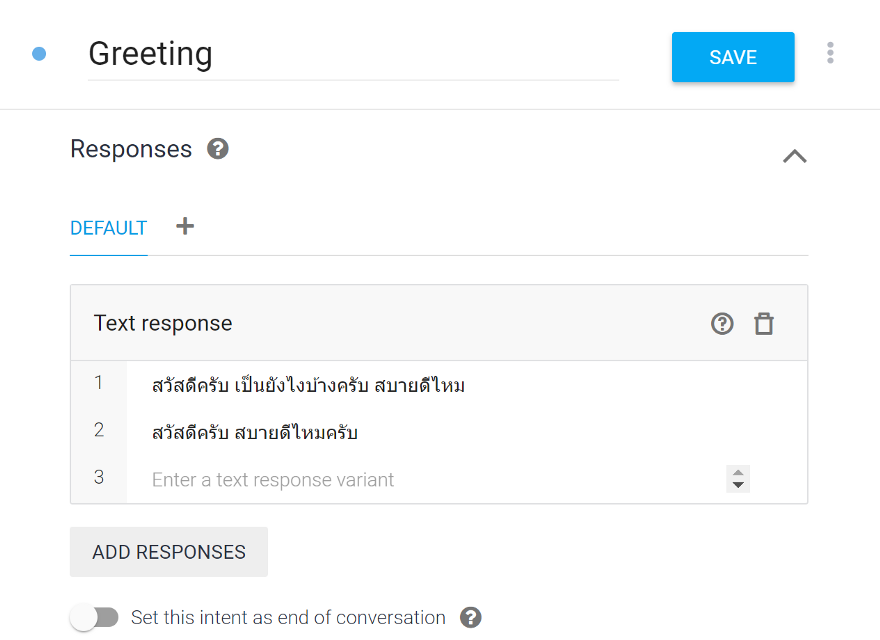
\includegraphics[width=0.9\columnwidth]{Figures/2/dialogflow_4}
		\caption{หน้า Intent ส่วน Responses}
		\label{Fig:dialogflow4}
	\end{figure}


ตรงส่วนของ Responses เราสามารถเพิ่มข้อความ หรือเพิ่ม balloon message ให้ต่อกันหลายๆอันได้ โดยกดที่ปุ่ม Add Responses และถ้าต้องการตั้งค่าว่า intent นี้เป็น intent สุดท้ายในการสนทนากัน ก็สามารถเปิด Checkbox Set this intent as end of conversation ซึ่งเดียวเราค่อนมาคุยกันแบบละเอียดอีกครั้ง ตอนที่ต้องทำ Contexts กันอีกครั้ง

\item ทดสอบคุยกับบอท \\
หลังจากเราลองทำ Greeting Intent เสร็จ ก็ถึงเวลาที่เราจะลองทดสอบการใช้งานกัน ซึ่งเราสามารถทดสอบได้ผ่านกล่องสนทนาที่อยู่ทางด้านขวา โดยลองพิมพ์คำว่า สวัสดี ลงไป ก็จะพบว่าแชทบอทจะตอบเรากลับมาว่า สวัสดีครับ เป็นยังไงบ้างครับ สบายดีไหม ตามที่เราตั้งค่าไว้ใน Responses นั้นเอง

	\begin{figure}[H]
		\centering
		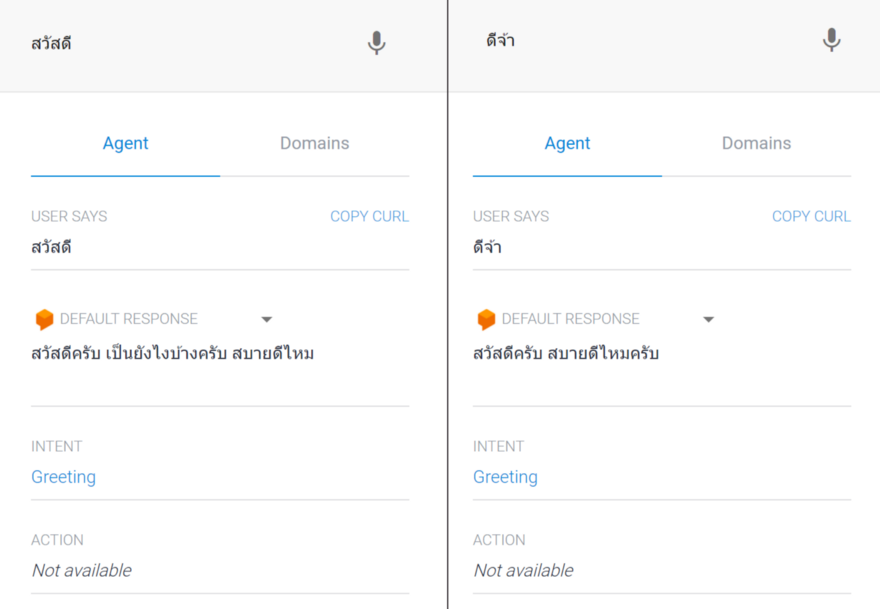
\includegraphics[width=0.9\columnwidth]{Figures/2/dialogflow_5}
		\caption{ทดสอบคุยกับบอท}
		\label{Fig:dialogflow5}
	\end{figure}

ถ้าดูจากภาพ \ref{Fig:dialogflow5} จะพบว่า ถ้าเราพิมพ์คำบางคำที่ไม่ได้มีอยู่ใน Training phrases อย่างคำว่า ดีจ้า ตัว Dialogflow ก็ฉลาดพอที่จะจับได้ว่านี่คือคำที่อยู่ในกลุ่มเดียวกับ สวัสดี ซึ่งเป็นคำทักทาย ที่เรากำหนดว่ามันคือ Intent Greeting นั้นเอง

แต่ในขณะเดียวกัน คำบางคำ หรือประโยคบางประโยคตัวแชทบอทของเราก็อาจจะยังไม่เข้าใจ ว่าสิ่งที่ผู้ใช้งานต้องการจะสื่อสารออกมา มันคือ Intent อะไร ซึ่งเวลาสร้าง Agent Dialogflow ก็จะสร้าง Default Fallback Intent ขึ้นมาให้ พร้อมกับ Responses บางส่วน ในกรณีที่แชทบอทไม่สามารถหา Intent ที่เหมาะสมได้ ก็จะมาตกที่เคสนี้ทั้งหมดตามภาพนั้นเอง

	\begin{figure}[H]
		\centering
		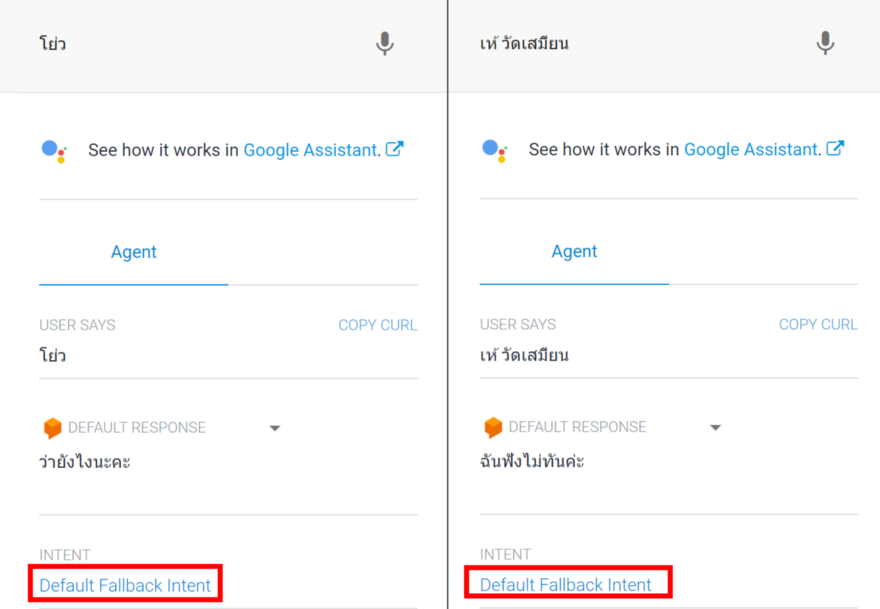
\includegraphics[width=0.9\columnwidth]{Figures/2/dialogflow_6}
		\caption{ทดสอบคุยกับบอท}
		\label{Fig:dialogflow6}
	\end{figure}

\end{enumerate}



\subsection{Libraries moment.js}
moment.js คือ javascript library สำหรับใช้สำหรับจัดการ Date และ Time ที่จะช่วยอำนวยความสะดวกในเรื่องการจัด Format Date ให้ตรงกับที่เราต้องการ
มี Feature ที่หลากหลายครอบคลุมทั้งใช้งาน Format ทั้ง Date , Time , Timezone , Standard Time , Local Time เป็นต้น ซึ่งการนำ library moment.JavaScript 
มาใช้งานสามารถติดตั้งได้ดังนี้

\subsubsection{คำสั่งในการติดตั้ง}
	\begin{figure}[H]
		{\setstretch{1.0}\begin{lstlisting}
/*  install dependency */
npm install moment --save   # npm
yarn add moment             # Yarn
Install-Package Moment.js   # NuGet
spm install moment --save   # spm
meteor add momentjs:moment  # meteor
bower install moment --save # bower (deprecated)
		\end{lstlisting}}
	\centering
		\caption{คำสั่งในการติดตั้ง moment.js}
		\label{Fig:momentjs}
	\end{figure}

\subsubsection{รูปแบบการใช้งาน moment.js}
	\begin{figure}[H]
		{\setstretch{1.0}\begin{lstlisting}
const moment = require('moment');

const SLASH_DMY = 'DD/MM/YYYY';
const SLASH_DMYHMS = 'DD/MM/YYYY HH:mm:ss';
const SLASH_YMD = 'YYYY/MM/DD';
const SLASH_YMDHMS = 'YYYY/MM/DD HH:mm:ss';
const DASH_DMY = 'DD-MM-YYYY';
const DASH_DMYHMS = 'DD-MM-YYYY HH:mm:ss';
const DASH_YMD = 'YYYY-MM-DD';
const DASH_YMDHMS = 'YYYY-MM-DD HH:mm:ss';
			
console.log('sysdate ::==',moment());
			
console.log('sysdate ::==',moment().format(SLASH_DMY));
console.log('sysdate ::==',moment().format(SLASH_DMYHMS));
			
console.log('sysdate ::==',moment().format(SLASH_YMD));
console.log('sysdate ::==',moment().format(SLASH_YMDHMS));
			
console.log('sysdate ::==',moment().format(DASH_DMY));
console.log('sysdate ::==',moment().format(DASH_DMYHMS));
			
console.log('sysdate ::==',moment().format(DASH_YMD));
console.log('sysdate ::==',moment().format(DASH_YMDHMS));
/*
sysdate ::== moment("2018-07-03T21:08:38.248")
sysdate ::== 03/07/2018
sysdate ::== 03/07/2018 21:08:38
sysdate ::== 2018/07/03
sysdate ::== 2018/07/03 21:08:38
sysdate ::== 03-07-2018
sysdate ::== 03-07-2018 21:08:38
sysdate ::== 2018-07-03
sysdate ::== 2018-07-03 21:08:38
*/
		\end{lstlisting}}
	\centering
		\caption{รูปแบบการใช้งาน moment.js}
		\label{Fig:howtomomentjs}
	\end{figure}

ทั้งหมดที่ยังไม่ใช้ทั้งหมดที่ Moment JS ทำได้ยังมีความสามารถอีกหลายอย่างที่ยังไม่ได้กล่าวถึงที่ Moment ทำได้เข้าไปดูได้ที่ https://momentjs.com/docs/

\subsection{Google Maps API}

Google Maps คือ บริการแผนที่ของ Google ซึ่งให้บริการ Services ที่เกี่ยวข้องกับแผนที่ทั้งหมด โดยในปัจจุบันแผนที่ของ Google
นั้นมีอยู่หลากหลายประเภท อาทิเช่นที่เราใช้บริการแผนที่บนเว็บไซต์ หรือ App บน Smartphone โดย Services เหล่านี้เราสามารถ
เรียกใช้ได้ฟรีในกรณีที่ผ่าน Application ทั่วไป แต่ถ้าในกรณีที่เราจะมีการเรียกใช้งานในเว็บไซต์หรือแอปพลิเคชันที่พัฒนาขึ้นเอง Google Maps 
ก็จะมี API ให้ใช้งานได้เช่นเดียวกัน แต่ Services ของ Google นั้นมีข้อจำกัดในการใช้งาน ถ้าต้องการใช้ในปริมาณที่สูงขึ้นก็จะต้องซื้อ Package 
ที่ทาง Google Maps มีมาให้ โดยปกติจะมีการจำกัดจำนวนที่ Request เข้ามาเรียกใช้งาน สำหรับเรียกใช้แผนที่และชุด service ต่าง ๆ ของ Google 
เพื่อพัฒนา Application ได้เหมือนกับ Google มีบริการ features ให้เรียกใช้ดังต่อไปนี้

	\begin{itemize}
		\item การปรับแต่งแผนที่ (Styled Map)
		\item ชุดควบคุมแผนที่ (Map Control)
		\item ชุดเครื่องมือวาดภาพบนแผนที่ (Drawing)
		\item การนำทางจากจุดหนึ่งไปยังอีกจุดหนึ่ง (Directions Service)
		\item การคำนวณความสูงของจุดพิกัด (Elevation Service)
		\item การแปลงที่อยู่เป็นพิกัด Lattitude เเละ Longtitude (GeoCoding Service)
		\item การดึงข้อมูล POI (Point of Interest)
		\item Street View
	\end{itemize}

	ประโยชน์ของการใช้งาน Google Maps

	\begin{itemize}
		\item สามารถค้นหาสถานที่ต่าง ๆ ได้อย่างสะดวกรวดเร็ว
		\item สามารถค้นหาชื่อถนนและสี่แยกได้
		\item สามารถค้นหาร้านอาหารในพื้นที่ที่ต้องการได้
		\item สามารถที่จะประชาสัมพันธ์สถานประกอบการทางธุรกิจ
		\item สามารถย่อหรือขยายแผนที่ทั่วโลกให้เล็กลงได้
		\item สามารถวางแผนเส้นทางการเดินทางไปยังพื้นที่ต่าง ๆ ได้
		\item สามารถใช้งานด้านระบาดวิทยาในการค้นหาแหล่งแพร่เชื้อ
		\item สามารถทำแผนที่หรือเส้นทางไปบ้านของตนเองได้
		\item สามารถแสดงตำแหน่งของตนเองได้
		\item สามารถดูและมองเห็นแผนที่ต่าง ๆ ทั่วโลกได้อย่างรวดเร็ว
	\end{itemize}

	การนำ Google Maps API มาใช้งาน

	สิ่งที่ต้องทำเพื่อเรียก Google Maps API มาใช้งานดังนี้
	\begin{enumerate}[label=\arabic*)]
		\item ทำการสมัครขอ API KEY โดยสามารถเข้าไปสมัครได้ที่ https://console.developers.google.com
		\item เพิ่มคำสั่งในบรรทัดที่ 2 ไว้ในไฟล์ index.html
		
		\begin{figure}[H]
			{\setstretch{1.0}\begin{lstlisting}
<head>
<script src="https://maps.googleapis.com/maps/api/js?key={API_KEY}" async defer></script>
</head>
		\end{lstlisting}}
	\centering
		\caption{เรียกใช้ API KEY}
		\label{Fig:googlemapapi}
	\end{figure}

	\item ขั้นตอนการเรียกใช้งานสำหรับแสดง Google Maps
	
	\begin{figure}[H]
		{\setstretch{1.0}\begin{lstlisting}
<-- IN HTML -->

<div #map id="map"></div> // เรียกใช้ map เพื่อแสดง

<-- IN TYPESCRIPT -->

map:any; //กำหนดตัวแปร map

ionViewDidLoad() {
  this.initMap();
} // เรียกใช้งานเมื่อหน้านี้ถูกเรียก

initMap() {
  this.map = new google.maps.Map(this.mapElement.nativeElement, {
    zoom: 7,
    center: {lat: 41.85, lng: -87.65}
  });
  this.directionsDisplay.setMap(this.map);
} // ฟังก์ชันสำหรับกำหนด map

<-- IN SCSS -->
	#map {
		height: 100%;
	} // ขนาดของ map
					
				\end{lstlisting}}
			\centering
				\caption{เรียกใช้งาน google maps ใน ionic framework}
				\label{Fig:googlemapionic}
			\end{figure}
			\item เรียกใช้งานด้วยคำสั่ง Google Maps เพื่อใช้งานตามต้องการ
		\end{enumerate}
		
	  

\section{เอกสารและงานวิจัยที่เกี่ยวข้อง}
\subsection{แอปพลิเคชันเครือข่ายสังคมออนไลน์เพื่อผู้สูงอายุ (OLDSTER) }
แอปพลิเคชันเครือข่ายสังคมออนไลน์เพื่อผู้สูงอายุ (OLDSTER) \cite{oldsterref} เป็นแอปพลิเคชันที่ถูกออกแบบมาเป็นเครือข่ายสังคมของผู้สูงอายุ โดยแอปพลิเคชันนี้ถูกออกแบบเพื่อผู้สูงอายุเป็นหลัก จึงง่ายต่อการใช้งาน มีรูปแบบที่ไม่ยุ่งยาก ไม่ซับซ้อน ตัวหนังสือเป็นแบบที่ง่ายต่อการอ่าน และขนาดไม่เล็กเกินไป 
มีฟังก์ชันการทำงาน 9 ฟังก์ชันดังนี้ ข้อมูลส่วนตัว กระดานข่าว พูดคุยระหว่างผู้ใช้งาน การแจ้งเตือน วิธีใช้งาน ข่าวสารในหมวดต่าง ๆ เป็นต้น โดยความแตกต่างระหว่างแอปพลิเคชัน OLDSTER กับ สูงวัยมายเฟรนด์ อยู่ตรงที่แอปพลิเคชันสูงวัยมายเฟรนด์
จะมีการให้ความรู้ในเรื่องโรคที่ผู้สูงอายุมักพบเจอในรูปแบบของแชทบอท และยังมีการแชทแบบกลุ่ม การค้นหาตำแหน่งของคนในครอบครัว รวมทั้งมีการแจ้งเตือนการทานยาอีกด้วย
\begin{figure}[H]
\centering
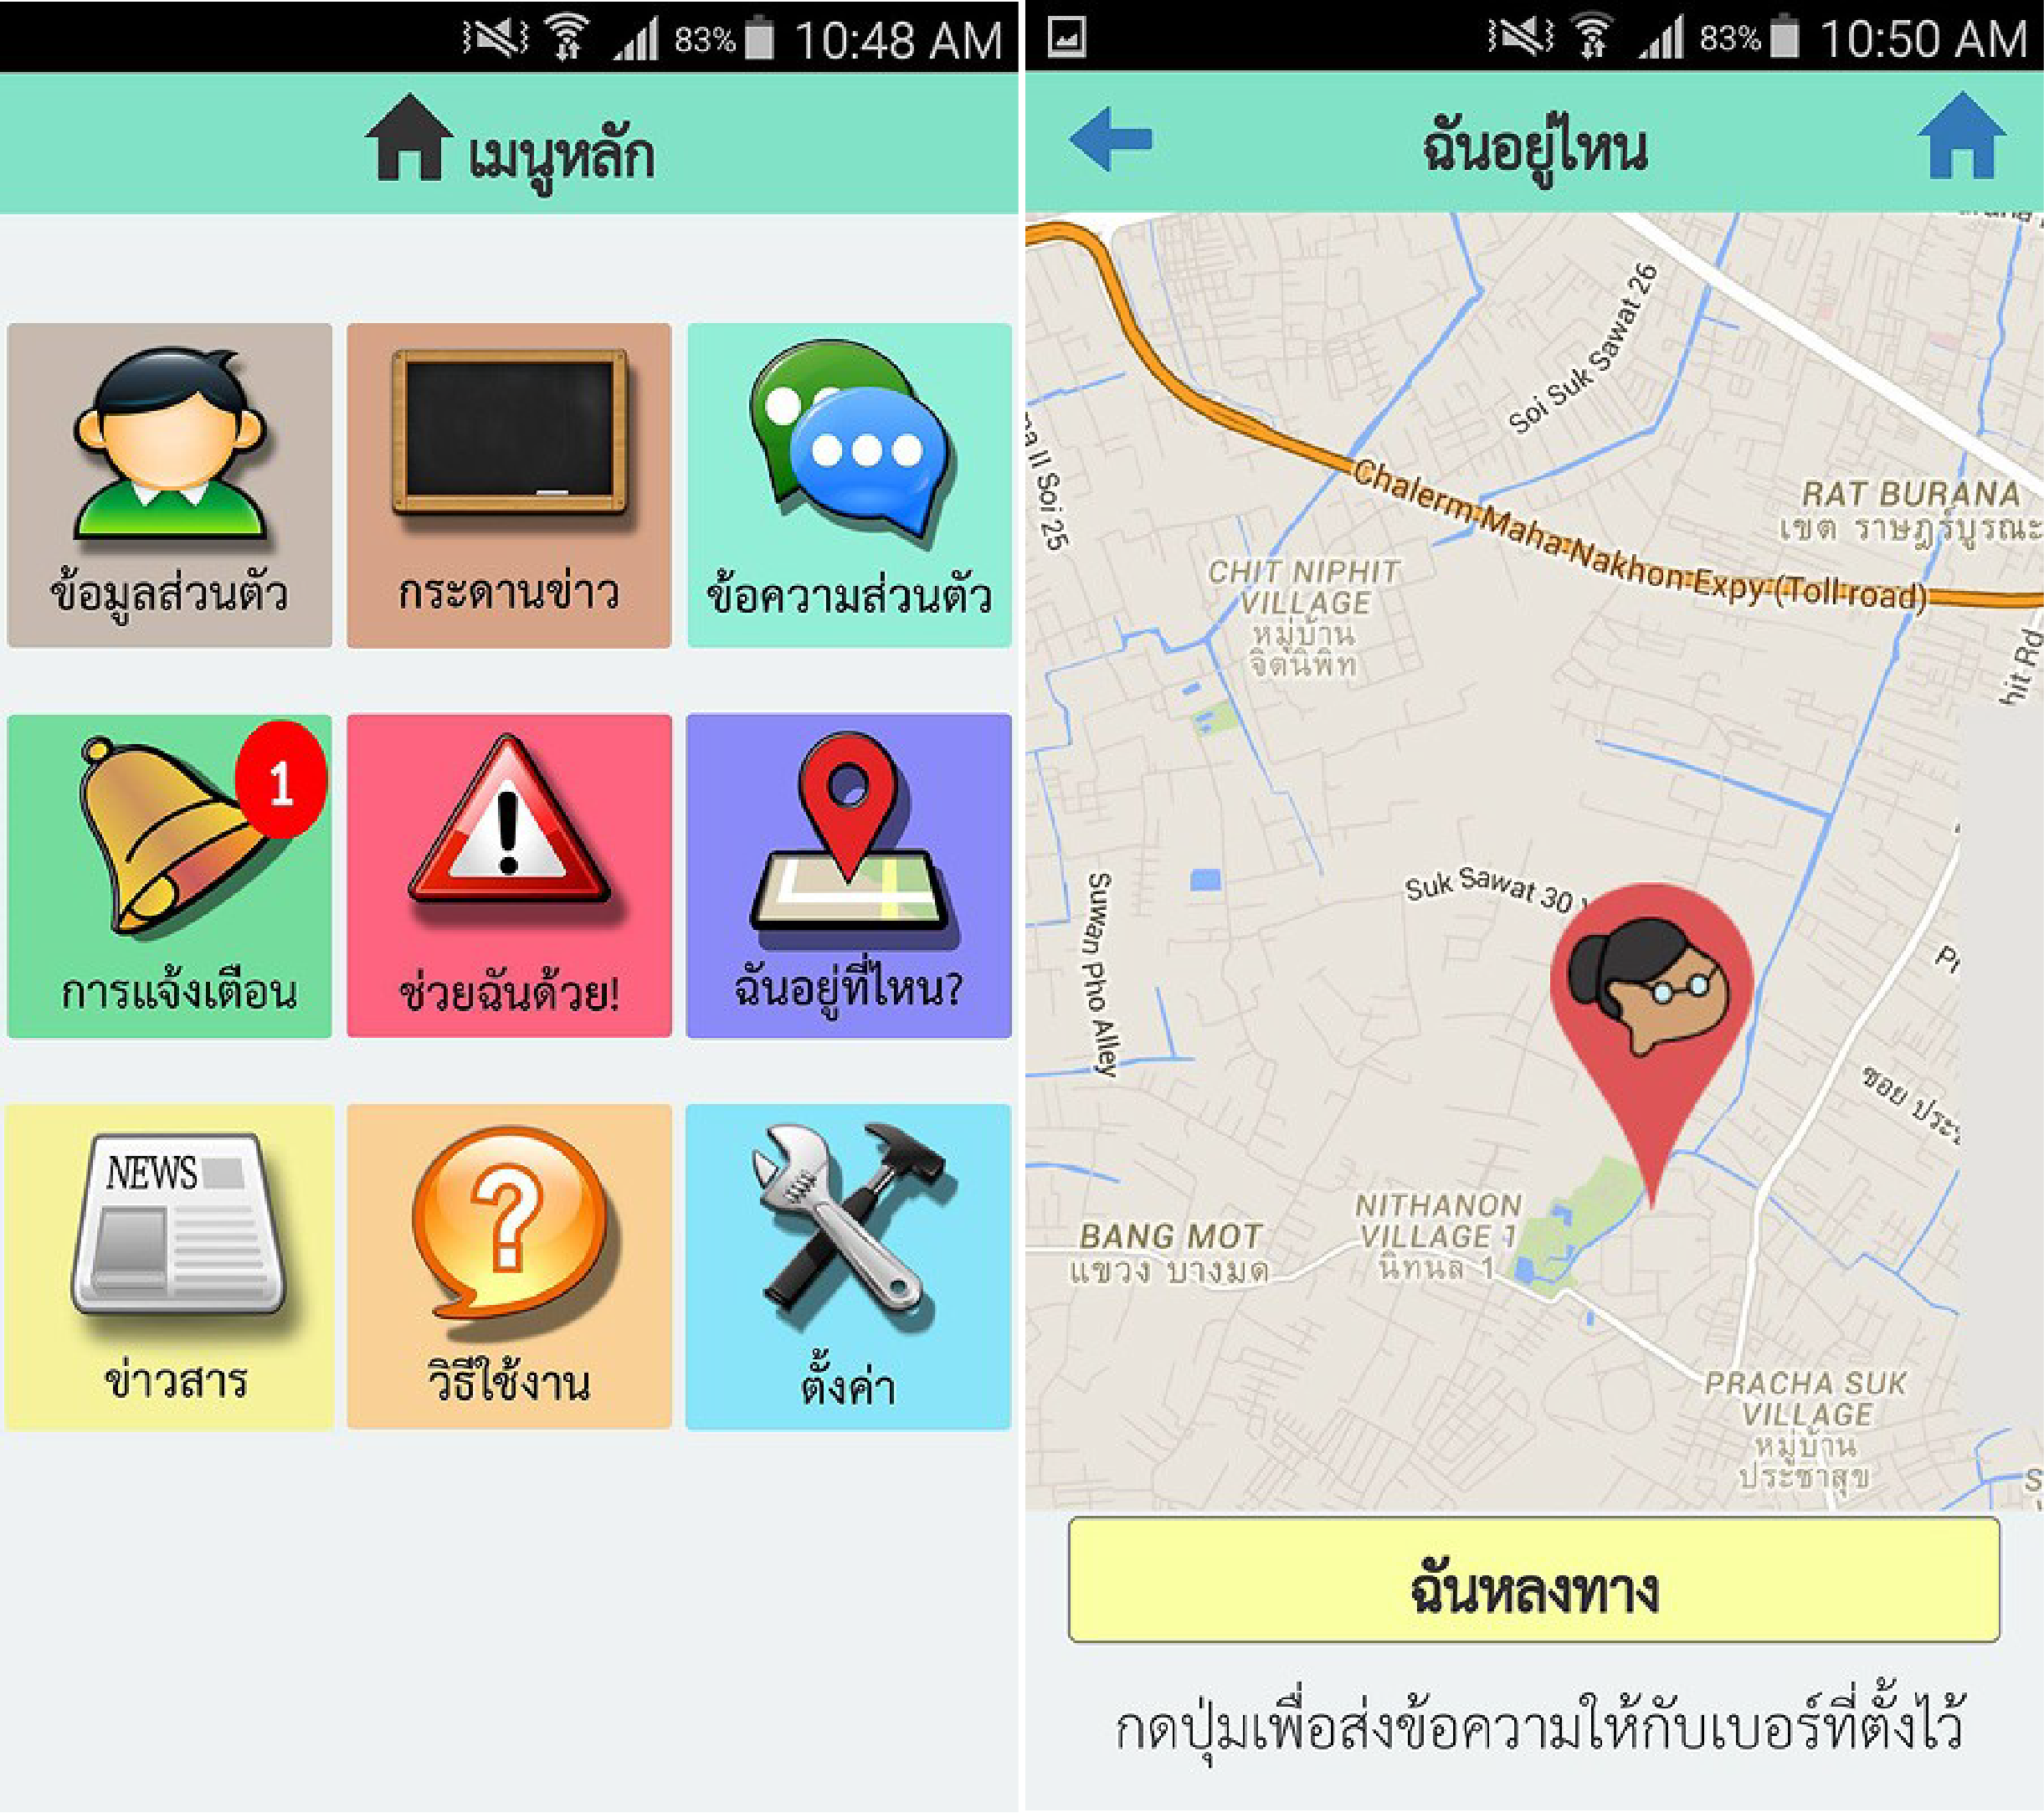
\includegraphics[width=0.8\textwidth]{Figures/2/oldsterfull}
\caption{แอปพลิเคชัน OLDSTER}
\label{Fig:ref1}
\end{figure}
	
\subsection{จับใจบอท}
จับใจบอท \cite{eStudentloan} เป็นแชทบอทที่สามารถพูดคุยได้ใน Messanger ของ Facebook เป้าหมายหลักคือเป็นแชทบอทที่ช่วยประเมินอาการซึมเศร้าของผู้ใช้งานได้ หากพบว่าตัวเองมีอาการซึมเศร้าก็จะช่วยในการตัดสินใจในการพบแพทย์ได้เร็วขึ้น 

\newpage
\begin{figure}[H]
	\centering
	
\includegraphics[width=0.8\textwidth]{Figures/2/ref2}
	\caption{แชทบอทของ จับใจบอท}{ที่มา : https://techsauce.co/tech-and-biz/jubjai-depression-detection-chatbot/}
	\label{Fig:ref2}
\end{figure}

ความแตกต่างระหว่าง จับใจบอท กับแอปพลิเคชันสูงวัยมายเฟรนด์ คือจับใจบอทเป็นการประเมินอาการซึมเศร้าเพียงอย่างเดียว ส่วนแอปพลิเคชันสูงวัยมายเฟรนด์จะแนะนำสาเหตุ และวิธีดูแลรักษาในเบื้องต้นให้แก่ผู้ใช้งาน


